\documentclass[master,euler,twoside,openright]{ustcthesis}
% 默认twoside 双面打印
% 将master修改为bachelor, doctor or master
% 要使用adobe字体,添加adobefonts选项
% 使用euler数学字体,如不愿使用,去掉euler
% 使用外文写作,请添加notchinese

% 设置图形文件的搜索路径
\graphicspath{{figures/}}

%仅用于本示例文档中显示特殊字符串
\usepackage{xltxtra}

%%%%%%%%%%%%%%%%%%%%%%%%%%%%%%
%% 封面部分
%%%%%%%%%%%%%%%%%%%%%%%%%%%%%%

  % 中文封面内容
  \title{基于演化算法的序回归\\技术研究}%一般情况下扉页和封皮、书脊共用一个标题文本,可以不用定义\spinetitle(仅硕博有用), \covertitle(本硕博均有用)和\encovertitle(仅本科有用)。特殊情况见下。
  \spinetitle{\small{基于演化算法的序回归技术研究\raisebox{-3pt}{(Beta)}}}
  %特殊情况1:本例中\title命令里含有换行控制字符,这会导致制作书脊的时候出现错误,例如如果你注释掉\spinetitle{...}这一行就会报错。这时需要定义一个不含换行等命令的\spinetitle,这并不表示\spinetitle里不能有任何命令——只能使用有限的命令。
  %特殊情况2:本例中标题过长,所以需要缩小书脊标题的字号。
  %特殊情况3:本例中中英文混排,由于tex竖排的原理限制,中英文基线不重合,所以需要人工调整英文的基线。具体调整量根据不同字体有所不同。
  \covertitle{基于演化算法的序回归\\技术研究}
  %\covertitle{中文题目第一行\\中文题目第二行}
  %不要在此调整封皮字体大小! Do not set Cover Page font size here!
  %特殊情况4:本例中\title中含有多个换行,导致标题超过了两行。根据制本厂规定,封皮标题不能超过两行。因此需要定义封皮使用的标题\covertitle. 如果你注释掉这一行,就会发现封皮不符合规定。
  \encovertitle{Ordinal Regression Techniques Based on Evolutionary Algorithms}
  %\encovertitle{English Title Line 1\\English Title Line 2\\English Title Line 3}
  %不要在此调整封皮字体大小! Do not set Cover Page font size here!
  %特殊情况5:仅本科生有用。本科封皮中有英文标题,不超过三行。与上类似。

  \author{伍\ 玉\ 舟}
  \depart{11系}%系别,硕博请用系代号,本科请用全称如
  %\depart{数理化和信息工程系}
  \major{计算机应用技术}%专业,硕博请用全称,本科不需要
  \advisor{唐珂\ 教授}
 % \coadvisor{冯晨珠\ 教授}%第二导师,没有请注释掉
  \studentid{SA13011013}%For bachelor only
  \submitdate{二〇一六年六月}

  % 英文封面内容
  \entitle{Ordinal Regression Techniques Based on Evolutionary Algorithms}
  \enauthor{Yuzhou Wu}
  \enmajor{Computer Technology and Applications}
  \enadvisor{Prof. Ke Tang}
  %\encoadvisor{Prof. Chenzhu Feng}%另外一个导师
  \ensubmitdate{June, 2016}

%%%%%%%%%%%%%%%%%%%%%%%%%%%%%%%%%%%%%%%%%%%%%%%%%%%%%%%%%%%%%%%%%%%%%
% If you use another language instead of chinese and english, then you
% should define some strings and provide information in your language.
%%%%%%%%%%%%%%%%%%%%%%%%%%%%%%%%%%%%%%%%%%%%%%%%%%%%%%%%%%%%%%%%%%%%%
%  \otherustcstr{zhong guo ke xue ji shu da xue}%A translation of `University of Science and Technology of China' in your language
%  \otherthesisstr{shuo shi xue wei lun wen}%A translation of `A dissertation for doctor(master/bachelor)'s degree' in your language
%  \otherauthorstr{xing ming}%A translation of `Author' in your language
%  \otherdepartmentstr{yuan xi}%A translation of `Department' in your language
%  \otherstudentidstr{xue hao}%A translation of `Student ID' in your language
%  \othersupervisorstr{dao shi}%A translation of `Supervisor' in your language
%  \otherfinishedtimestr{ri qi}%A translation of `Finished Time' in your language
%  \otherspecialitystr{zhuan ye}%A translation of `Speciality' in your language
%  \othertitle{zhong guo ke xue ji shu da xue tong yong xue wen lun wen shi li wen dang}
%  \otherauthor{zhao qian sun}
%  \otheradvisor{zhou wu zheng}
%  \othercoadvisor{feng chen zhu}
%  \othersubmitdate{hou nian ma yue}
%  \othermajor{mou zhuan ye}
%  \otherdepart{mou xi}

\begin{document}

  % 封面
  \maketitle

%特别注意,以下述顺序为准,在对应部分添加文档部件,切勿颠倒顺序:
%本科论文的文档部件顺序是:
%    frontmatter:致谢、目录、中文摘要、英文摘要、
%    mainmatter: 正文章节
%    backmatter: 参考文献或资料注释、附录
%硕博论文的文档部件顺序是:
%    frontmatter:中文摘要、英文摘要、目录、符号说明
%    mainmatter: 正文章节
%    backmatter: 参考文献、附录、致谢、发表论文
%%%%%%%%%%%%%%%%%%%%%%%%%%%%%%
%% 前言部分
%%%%%%%%%%%%%%%%%%%%%%%%%%%%%%
\frontmatter
\makeatletter
\ifustc@bachelor
	%%%%%%%%%%%%%%%%%
	%本科论文修改这里
	%%%%%%%%%%%%%%%%%
	% 致谢
	
\begin{thanks}

首先,感谢我的导师唐珂教授在三年研究生生涯里对我的悉心指导和教诲。唐老师严谨踏实、勇于创新的科研作风深深影响了我。在此,我诚挚地向唐老师表示衷心的感谢。

此外,感谢孙宇、梁新乐、王娟、李丙栋等师兄师姐们对我的指点和照顾;感谢李皈颖、张良鹏、沈汪洋等几位同学,与你们讨论交流让我受益良多;感谢付嘉懿、刘晟才、魏羽凡、刘俊龙等师弟师妹,我们在UBRI实验室共同学习共同生活,一起走过了这段愉快而难忘的岁月。

感谢科大,提供如此淳朴、安静而美丽的校园环境让我学习和成长。

最后,感谢家人对我的支持和鼓励。

\vskip 18pt

\begin{flushright}

~~~~伍玉舟~~~~

\today

\end{flushright}

\end{thanks}

	
	%目录部分
	%目录
	\tableofcontents
	%默认表格、插图、算法索引名称分别为“表格索引”、“插图索引”和“算法索引”
	%如果需要自行修改lot,lof,loa的名称,请定义
	%\ustclotname{...}
	%\ustclofname{...}
	%\ustcloaname{...}

	% 表格索引
	\ustclot
	% 插图索引
	\ustclof
	%算法索引
	%如果需要使用算法环境并列出算法索引,请加入补充宏包。
	\ustcloa
	
	% 摘要
	
\begin{cnabstract}
本文是中国科学技术大学本硕博毕业论文模板示例文件。本模板由ywg@USTC创建,适用于撰写学士、硕士和博士学位论文,本模板由原来的本科模板和硕博模板整合优化而来。本示例文件除了介绍本模板的基础用法外,本文还是一个简要的学位论文写作指南。

\keywords{中国科学技术大学,学位论文,\LaTeX{}~通用模板,学士,硕士,博士}
\end{cnabstract}


\begin{enabstract}

This is USTC thesis template for bachelor, master and doctor user's guide. The template is created by ywg@USTC and a derivative of USTC Bachelor and Master-PhD templates. Besides that
the usage of the template, a brief
guideline for writing thesis is also provided.


\enkeywords{University of Science and Technology of China (USTC), Thesis, Universal \LaTeX{} Template, Bachelor, Master, PhD}
\end{enabstract}
%此文件中含有中英文摘要
\else
	%%%%%%%%%%%%%%%%%
	%硕博论文修改这里
	%%%%%%%%%%%%%%%%%
	% 摘要
	
\begin{cnabstract}
本文是中国科学技术大学本硕博毕业论文模板示例文件。本模板由ywg@USTC创建,适用于撰写学士、硕士和博士学位论文,本模板由原来的本科模板和硕博模板整合优化而来。本示例文件除了介绍本模板的基础用法外,本文还是一个简要的学位论文写作指南。

\keywords{中国科学技术大学,学位论文,\LaTeX{}~通用模板,学士,硕士,博士}
\end{cnabstract}


\begin{enabstract}

This is USTC thesis template for bachelor, master and doctor user's guide. The template is created by ywg@USTC and a derivative of USTC Bachelor and Master-PhD templates. Besides that
the usage of the template, a brief
guideline for writing thesis is also provided.


\enkeywords{University of Science and Technology of China (USTC), Thesis, Universal \LaTeX{} Template, Bachelor, Master, PhD}
\end{enabstract}
%此文件中含有中英文摘要
	% 目录
	\tableofcontents
	%默认表格、插图、算法索引名称分别为“表格索引”、“插图索引”和“算法索引”
	%如果需要自行修改lot,lof,loa的名称,请定义
	%\ustclotname{...}
	%\ustclofname{...}
	%\ustcloaname{...}

	% 表格索引
	\ustclot
	% 插图索引
	\ustclof
	%算法索引
	%如果需要使用算法环境并列出算法索引,请加入补充宏包。
	\ustcloa
	
	%符号说明,需要加入补充包
	%\begin{denotation}

\item[HPC] 高性能计算 (High Performance Computing)
\item[cluster] 集群
\item[Itanium] 安腾
\item[SMP] 对称多处理
\item[API] 应用程序编程接口
\item[PI]	聚酰亚胺
\item[MPI]	聚酰亚胺模型化合物,N-苯基邻苯酰亚胺
\item[PBI]	聚苯并咪唑
\item[MPBI]	聚苯并咪唑模型化合物,N-苯基苯并咪唑
\item[PY]	聚吡咙
\item[PMDA-BDA]	均苯四酸二酐与联苯四胺合成的聚吡咙薄膜
\item[$\Delta G$]  	活化自由能~(Activation Free Energy)
\item [$\chi$] 传输系数~(Transmission Coefficient)
\item[$E$] 能量
\item[$m$] 质量
\item[$c$] 光速
\item[$P$] 概率
\item[$T$] 时间
\item[$v$] 速度
\end{denotation}
%不是必需的,如果不想列出请注释掉
\fi
\makeatother

%%%%%%%%%%%%%%%%%%%%%%%%%%%%%%
%% 正文部分
%%%%%%%%%%%%%%%%%%%%%%%%%%%%%%
\mainmatter

  
\chapter{绪论}
\label{chap:introduction}

序回归问题作为机器学习领域里一个比较有代表性的问题,它和传统的分类问题、回归问题都有一定的相似性。本章将首先介绍序回归问题的特点,以及与之相关的一些实际应用。其次,在文献综述中将简单将介绍处理序回归问题的常用方法。最后,我们将概述本文的研究内容和主要贡献。

\section{研究内容背景及意义}
\label{intro_back}
在许多实际应用中,数据的不同类别之间存在一个自然的序关系。例如,消费者在评价服务质量时,会使用“非常不满意”、“不满意”、“一般”、“满意”、“非常满意”等来描述自己的感受。这些不同的描述之间存在一个自然的序关系。相对于标称数据(norminal data),这种类型的数据称为有序数据(ordinal data)。有序数据具有以下一些特点:
\begin{enumerate}
\item[1.] 有序数据的类别之间可以做一个排序。在这个例子当中,按照消费者的评价由坏到好,依次为“非常不满意”、“不满意”、“一般”、“满意”、“非常满意”,则其对应的序(rank)依次为1到5。这里的序指的是该类别在所有类别中所处的位置,在序回归问题中,通常我们也使用“序”来指相应的类别。
\item[2.] 通常情况下,有序数据的序的个数(即类别的个数)是有限的。例如在这个消费者评价服务质量的应用中,共有5个序。
\item[3.] 类别之间的差别没有精确的定义。例如,我们不知道“满意”比“一般”究竟好多少,也不知道“非常满意”的一半是否等价于“满意”。
\end{enumerate}
预测这种有序数据的序的学习问题就称为序回归(ordinal regression)。序回归有着广泛的实际应用场景。金融行业经常需要对用户进行信用评级:应用场景里给定一些用户的属性数据(性别、年龄、收入、历史消费记录等)以及相应的信用等级,假设信用等级从低到高有三个类别,依次为1、2、3。使用已有的用户数据可以建立一个信用评级模型,当需要对一个新用户进行信用评价时,向模型输入该用户的属性数据,输出信用等级。可以看到,信用等级具有明显的序关系,因此这可以作为一个典型的序回归问题来处理\citep{kwon1997ordinal}\citep{kim2012corporate}\citep{dikkers2005support}\citep{fernandez2013addressing}。
%[Y. Kwon, I. Han and K. Lee, "Ordinal pairwise partitioning (OPP) approach to neural networks training in bond rating,"Intell. Syst. Accounting Finance Manag., vol. 6, no. 1, pp. 23-40, 1997 [CrossRef] 
%K.-j. Kim and H. Ahn, "A corporate credit rating model using multi-class support vector machines with an ordinal pairwise partitioning approach,"Comput. Oper. Res., vol. 39, no. 8, pp. 1800-1811, 2012 [CrossRef] 
%H. Dikkers and L. Rothkrantz, "Support vector machines in ordinal classification: An application to corporate credit scoring,"Neural Netw. World, vol. 15, no. 6, pp. 491-507, 2005
%F. Fernández-Navarro, P. Campoy-Muõoz, M.-D. La Paz-Marín, C. Hervás-Martínez and X. Yao, "Addressing the EU sovereign ratings using an ordinal regression approach,"IEEE Trans. Cybern., vol. 43, no. 6, pp. 2228-2240, 2013]
此外,序回归还应用在情感分析、信息检索、推荐系统、心理学、医学\citep{bender1997ordinal}\citep{bender1998using}\citep{jang2011effect}\citep{doyle2014predicting}\citep{perez2011ordinal}\citep{cardoso2005modelling}\citep{perez2014organ}等领域。
%[R. Bender and U. Grouven, "Ordinal logistic regression in medical research,"J. R. Coll. Phys. Lond., vol. 31, no. 5, pp. 546-551, 1997
%R. Bender and U. Grouven, "Using binary logistic regression models for ordinal data with non-proportional odds,"J. Clin. Epidemiol., vol. 51, no. 10, pp. 809-816, 1998 [CrossRef] 
%W. M. Jang, S. J. Eun, C.-E. Lee and Y. Kim, "Effect of repeated public releases on cesarean section rates,"J. Prev. Med. Pub. Health, vol. 44, no. 1, pp. 2-8, 2011 [CrossRef] 
%O. M. Doyle, E. Westman, A. F. Marquand, P. Mecocci, B. Vellas, M. Tsolaki, I. Kłoszewska, H. Soininen, S. Lovestone, S. C. Williams and A. Simmons, "Predicting progression of alzheimers disease using ordinal regression,"PloS one, vol. 9, no. 8, pp. e105542, 2014 [CrossRef] 
%M. Pérez-Ortiz, P. A. Gutiérrez, C. García-Alonso, L. Salvador-Carulla, J. A. Salinas-Pérez and C. Hervás-Martínez, "Ordinal classification of depression spatial hot-spots of prevalence,"Proc. 11th Int. Conf. Intell. Syst. Des. Appl., pp. 1170-1175, 2011
%J. S. Cardoso, J. F. P. da Costa and M. Cardoso, "Modelling ordinal relations with SVMs: An application to objective aesthetic evaluation of breast cancer conservative treatment,"Neural Netw., vol. 18, no. 5/6, pp. 808-817, 2005 [CrossRef] 
%M. Pérez-Ortiz, M. Cruz-Ramírez, M. Ayllón-Terán, N. Heaton, R. Ciria and C. Hervás-Martínez, "An organ allocation system for liver transplantation based on ordinal regression,"Appl. Soft Comput. J., vol. 14, pp. 88-98, 2014 [CrossRef] 

%此处可以加上一些实际的例子,或者引用
%TKDE2016 Some of the fields where ordinal regression is found are medical research [5], [6], [7], [8], [9], [10], [11], age estimation [12], brain computer inter- face [13], credit rating [14], [15], [16], [17], econometric modelling [18], face recognition [19], [20], [21], facial beauty assessment [22], image classification [23], wind speed pre- diction [24], social sciences [25], text classification [26], and more. 

%引入这个序信息往往会导致问题是非凸、不可导,或者没有明确的数学形式,而演化算法(EA) 能够帮助我们更好地处理序回归问题。

\section{文献综述及研究成果}
%可以写一些序回归研究的历史
%写OR和learning to rank, preference learning, sorting 等问题的不同
在早期的机器学习工作当中,研究者并不考虑类别之间的序关系,因此在处理序回归问题时,仅当做传统的分类问题来处理。序回归问题从2000年左右开始,逐渐受到研究者的关注,并涌现了许多序回归技术。

在序回归问题中,由于序的个数是有限的,所以序回归和传统分类问题有一定的相似性。此外,数据的类别之间是有序的,所以序回归和传统的回归问题也有一定的相似性。对于这两方面的相似性,研究者分别从两个角度考虑了如何更好地处理序回归问题。从分类的角度来说,直接使用传统的分类技术来处理序回归问题会忽略数据本身所具有的序信息,而这个序信息提供了一种先验信息,忽略这个信息会使得结果并不理想。从回归的角度来说,有序数据比传统的回归数据更复杂,不同类别之间虽然有序,但是这个序却不能准确地度量类别之间的差别,这使得数据分布更不规则,从而比传统的回归问题更难处理。因此,为了更好地处理序回归问题,我们需要设计专门的序回归技术,而不能仅仅直接使用传统的分类、回归技术。如何使用序信息,从而达到比传统分类、回归技术更优的效果,将是研究序回归问题的一个重点,同时也是难点。此外,在数据量日益增加的今天,很多实际应用需要获取大量的标签数据,而获取标签将耗费大量的人力、物力。因此,如何使用大量存在的无标签数据将具有重要的研究价值。在序回归问题中,随着序个数的增加,有监督学习模型将需要更多有标签数据来确定不同序的类别之间的边界。对于这个挑战,已有一些研究者提出了半监督序回归技术。我们将在第二章中详细介绍序回归技术的发展历程和已有的研究成果,并指出其中不足。本文将以此为切入点,提出我们对于序回归问题所做的一些探索和研究成果。

% 详细介绍演化算法

%In ordinal regression, the labels of data not only show the categories they belong to but also indicate their ranks in the whole data set. Therefore, it is more challenging to use the unlabeled data in this learning task. Specifically, due to the need for including the order information, it is difficult to estimate the potential distribution of ordinal data accurately. Besides, the models are usually non- convex and non-differentiable after involving the unlabeled data, since a rank constraint is typically employed to preserve the order information (e.g., see the models in [5, 7]).

\section{本文概述及主要贡献}
\subsection{本文研究内容}
本文首先回顾并梳理序回归技术的发展历程,分别从基于有监督学习方式的序回归技术、基于半监督学习方式的序回归技术、基于演化算法的序回归技术三个大类入手,介绍一些有代表性的算法,并总结发展趋势及不足之处。对有监督序回归技术的研究时间较长、较为深入,而对半监督序回归技术的研究尚浅,近几年才出现一些。在序回归中,数据的标签不仅体现它所属的类别,同时也表示了它在整个数据集上的序信息。因此,相比较于传统的分类问题,序回归中的无标签数据缺失了更多的信息,如何在半监督学习方式下使用无标签数据将更具挑战性。针对该难点,本文提出了一种有效的基于半监督学习方式的序回归技术——基于加权核判别分析的半监督序回归技术(WKFDOR\citep{wu2015evolutionary})。
%Wu Y, Sun Y, Liang X, et al. Evolutionary semi-supervised ordinal regression using weighted kernel Fisher discriminant analysis[C]//Evolutionary Computation (CEC), 2015 IEEE Congress on. IEEE, 2015: 3279-3286.
此外,为了更有效地利用无标签数据和序信息,本文又在WKFDOR算法的基础上做了改进,提出了基于演化算法的半监督序回归技术(ESSOR\citep{wu2015evolutionary})。通过对比实验,我们验证了提出的算法能够有效地利用无标签数据提升处理序回归问题的效果。

\subsection{本文主要贡献}
本文的主要贡献包括如下几点:
主要针对已有序回归技术研究中的不足,做出了以下几点贡献:
\begin{enumerate}
\item[1.]梳理并总结了序回归技术的发展,指出其中待完善之处。
\item[2.]提出了一种有效的半监督序回归技术,能够利用无标签数据提升处理序回归问题的效果。
\item[3.]提出了一种基于演化算法的半监督序回归技术,通过演化算法的迭代优化过程,更有效地利用了无标签数据以及序信息。
%[wu等人 引用essor]本文首次提出了基于演化算法的半监督序回归技术,其效果显著。
\item[4.]近年来,有相当多的将演化算法和机器学习结合起来的工作,并取得了积极的结果。本工作也是将演化算法和机器学习结合起来,是对这二者结合使用的一个很好的实例研究。
\end{enumerate}

\subsection{本文结构}
第二章回顾了序回归技术的发展;第三章研究了半监督序回归问题,并提出了半监督序回归技术——WKFDOR;第四章在第三章的基础上做了改进,提出了基于演化算法的半监督序回归技术——ESSOR;第五章总结了本文的研究工作并提出了未来的研究方向。

  \chapter{序回归技术发展回顾}
\label{chap:review}
序回归问题在过去十几年的时间里,受到了研究者的广泛关注,涌现了一系列序回归技术。本章将对序回归技术的发展做回顾,对已有的比较有代表性的研究成果根据方法的特点进行分类。首先我们将给出序回归问题的形式化定义,以及常用的算法评估指标。接着我们从三个方向分别回顾已有的序回归技术:基于有监督学习方式的序回归技术、基于半监督学习方式的序回归技术、基于演化算法的序回归技术。最后我们总结了序回归技术发展的趋势和不足。

\section{序回归问题定义和评估指标}
%对于一个输入的属性特征向量\(x\),序回归问题是要预测\(x\)的标签\(y\),其中
考虑一个有\(K\)个有序类别的序回归问题,这\(K\)个类别(序)用一个连续的整数集合 \(Z=\{1,2,\dots,K\}\)来表示,整数的值表示相应类别在整个标签集合中的序。给定一个包含\(N\)个样例(instances)的训练集合(training set),其中可能包含有标签数据和无标签数据。样例的属性特征向量\(x_{i} \in \chi \subseteq R^{d}\),有标签样例的标签\(y_{i} \in Z\)。问题的目标是用训练集学习到一个序回归模型,该模型可以对测试样例(testing instance)给出一个预测的标签。需要指出的是,这里的测试样例是在训练过程中未曾出现的新样例。

%丰富metric的已有研究

假设序回归模型对测试集预测的标签是\(\{\hat{y_{1}},\hat{y_{2}},\dots,\hat{y_{t}}\}\),而测试集的真实标签是 \(\{y_{1},y_{2},\dots,y_{t}\}\) ,通常采用下面两种指标来评估模型的性能:
\begin{enumerate}
\item[1.] \textit{Mean absolute error}: \(MAE=\frac{1}{t}\sum_{i=1}^{t}|\hat{y_{i}}-y_{i}|\), 用来量化预测标签和真实标签之间偏差的平均值。
\item[2.] \textit{Mean zero-one error}: \(MZE=\frac{1}{t}\sum_{i=1}^{t}\mathbb{I}(\hat{y_{i}}\neq y_{i}) = 1-Acc\),其中\(\mathbb{I}(\cdot)\)是指示函数。\(MZE\)用来量化模型的错误率(error rate)。
\end{enumerate}

\section{基于有监督学习方式的序回归技术}
% 从篇幅角度考虑加上用回归来做的方法综述
在机器学习里,通常使用已知真实标签的样例去训练模型,再用训练好的模型去预测新样例的标签。这种学习方式称作有监督学习。在序回归问题的研究中,基于有监督学习方式的序回归技术已有相当长的研究历史。下文我们将基于有监督学习方式的序回归技术简称为有监督序回归技术。

根据方法的特点,我们可以大致将已有的有监督序回归技术分成三类:
\begin{enumerate}
\item[1.]第一类方法将序回归问题当作传统的标称分类问题(nominal classification problem)或者传统的回归问题(regression problem),使用已有的分类或回归方法来处理。
\item[2.]第二类方法先将序回归问题分解成多个二分类问题(binary classification problem),再使用传统的分类模型来处理每个子问题,最后对子问题的结果进行合并得到原问题的结果。通过设计的分解策略,序回归问题中的序信息可以保留下来。
\item[3.]第三类方法通过拓展传统的分类模型来使序信息可以加入到模型学习中,例如显式增加一个序关系约束条件。这种方法相比较于前两种方法,对序信息的处理更加直接,通常效果也更好。因此本节着重介绍了第三类方法。
\end{enumerate}

下面将分别介绍这三类有监督序回归技术。

%\subsection{有监督序回归问题定义}
%考虑一个有\(K\)个类别的序回归问题,该问题的目标是预测一个输入向量\(x\in \chi \subseteq R^{d}\)的标签(label)\(y\in \)

%考虑一个有\(K\)个有序类别的序回归问题,这\(K\)个类别(序)用一个连续的整数集合 \(Z=\{1,2,\dots,K\}\)来表示,整数的值表示相应类别在整个标签集合中的序。在有监督序回归问题中,给定一个包含\(L\)个有标签样例(instances)的训练集合(training set)\((X^{l},Y^{l})=\{(x_{1:L},y_{1:L})\}\),其中\(x_{i} \in \chi \subseteq R^{d}\),\(y_{i} \in Z\)。问题的目标是用训练集学习到一个序回归模型,该模型可以对测试样例(testing instance)给出一个预测的标签。

\subsection{直接用传统分类或回归方法处理的序回归技术}
由于序回归问题兼具传统分类和回归问题的特性,所以经常会直接用传统的分类或回归技术来处理序回归问题。

从回归的角度来考虑,可以将序回归的标签转化成一些实数值\citep{torra2006regression},
%[V. Torra, J. Domingo-Ferrer, J. M. Mateo-Sanz and M. Ng, "Regression for ordinal variables without underlying continuous variables,"Inf. Sci., vol. 176, no. 4, pp. 465-474, 2006]
然后使用标准的回归技术\citep{bishop2006pattern}\citep{murphy2012machine}
%[C. M. Bishop, Pattern Recognition and Machine Learning, 2007, Springer]
%[Murphy K P. Machine learning: a probabilistic perspective[M]. MIT press, 2012.]
来处理(例如,支持向量回归、树模型、神经网络等)。例如,Kramer等人\citep{kramer2001prediction}
%[S. Kramer, G. Widmer, B. Pfahringer and M. D. Groeve, "Prediction of ordinal classes using regression trees,"Fundamenta Inf., vol. 47, no. 1-2, pp. 1-13, 2001]
通过给序附上特定的数值,应用树模型来学习,在预测新样例时,通过四舍五入树模型得到的实数值给出新样例的标签。在\autoref{intro_back}中,我们分析了序回归问题的特点之一是类别之间的差别没有精确的定义,所以这类方法的一个主要问题是很难在没有先验知识的情况下对标签进行准确的度量。

从分类的角度来考虑,当我们不考虑类别之间的序关系时,序回归问题就是一个传统的标称分类问题。有一些研究者直接使用传统的标称分类模型(例如,支持向量机、决策树、罗辑思特回归等)来处理序回归问题,由于忽略了数据中的序信息,使得问题的难度有所增加,往往需要更多的训练数据。此外,序信息可以被理解为一种先验知识,合理地利用序信息能够有效地提升预测效果。因此,出现了第三类序回归技术,即在传统的分类模型下引入序信息,这将在后面小节中介绍。

另一种更精细的做法是使用代价敏感的分类技术来处理序回归问题。其主要做法是引入一个代价矩阵(cost matrix),对不同的错分给予不同的代价。例如,将序为\(1\)的标签预测成序为\(3\)的标签,其代价要大于预测成序为\(2\)的标签。Kotsiantis和Pintelas\citep{kotsiantis2004cost}
%[S. B. Kotsiantis and P. E. Pintelas, "A cost sensitive technique for ordinal classification problems,"Proc. Methods Appl. Artif. Intell. (Proc. 3rd Hellenic Conf. Artif. Intell.), pp. 220-229, 2004 [CrossRef]]
使用绝对值代价矩阵来处理序回归问题。假设真实标签的序为\(i\),将其错误地预测为序是\(j\)的标签,则相应的绝对值代价\(c = \left |  i - j \right |\)。\autoref{table_costMat}列出了几种常见的代价矩阵形式,其中矩阵的列是真实标签,行是预测的标签。设计不同的代价矩阵,将对结果产生不同的影响。这种方法的主要问题和用传统回归技术来处理的方式相似,即在没有先验知识的情况下我们很难定义一个合适的代价矩阵。

\begin{table}[!htbp]
\caption{5类别序回归问题的不同代价矩阵举例}
\label{table_costMat}
\centering
\begin{tabular}{ccc}
\toprule
绝对值代价 & 0-1代价 & 二次方代价 \\
\midrule
$ \left[
 \begin{matrix}
   0 & 1 & 2 & 3 & 4 \\
   1 & 0 & 1 & 2 & 3 \\
   2 & 1 & 0 & 1 & 2 \\
   3 & 2 & 1 & 0 & 1 \\
   4 & 3 & 2 & 1 & 0 \\
  \end{matrix}
  \right]
$

&

$ \left[
 \begin{matrix}
   0 & 1 & 1 & 1 & 1 \\
   1 & 0 & 1 & 1 & 1 \\
   1 & 1 & 0 & 1 & 1 \\
   1 & 1 & 1 & 0 & 1 \\
   1 & 1 & 1 & 1 & 0 \\
  \end{matrix}
  \right]
$

&

$ \left[
 \begin{matrix}
   0 & 1 & 4 & 9 & 16 \\
   1 & 0 & 1 & 4 & 9  \\
   4 & 1 & 0 & 1 & 4 \\
   9 & 4 & 1 & 0 & 1 \\
   16 & 9 & 4 & 1 & 0 \\
  \end{matrix}
  \right]
$
\\
\bottomrule
\end{tabular}
\end{table}

\subsection{先分解成二分类问题再进行处理的序回归技术}
序信息的存在使得我们能够直观地比较两个不同的标签。对于一个给定的序\(q\),一个直接的问题就是,“样例\(x\)的标签的序是否大于\(q\)?”\citep{lin2012reduction}。
%[H.-T. Lin and L. Li, "Reduction from Cost-sensitive ordinal ranking to weighted binary classification,"Neural Comput., vol. 24, no. 5, pp. 1329-1367, 2012 [CrossRef] ]。
很显然,这是一个二分类问题。因此,为了引入序信息,一些研究提供了一种思路,即先将原问题分解成多个二分类问题,再使用传统的分类技术来处理这些二分类问题,最终将二元输出组合成标签。通过设计的分解策略(编码策略),原问题的序信息可以保存下来。

Frank和Hall\citep{frank2001simple}
%[E. Frank and M. Hall, “A simple approach to ordinal classifica- tion,” in Proceedings of the European Conference on Machine Learning. Springer Berlin Heidelberg, 2001, pp. 145–156.] 
提出了一种叫OrderedPartitions的分解方法,并使用C4.5来处理每个二分类问题,最后通过概率的形式得到最终的结果。还有一些其它的分解策略被提出来\citep{kwon1997ordinal}
%[Y. Kwon, I. Han and K. Lee, "Ordinal pairwise partitioning (OPP) approach to neural networks training in bond rating,"Intell. Syst. Accounting Finance Manag., vol. 6, no. 1, pp. 23-40, 1997]
,见\autoref{table_decMat}。其中矩阵的每一列对应一个二分类子问题,行对应每个类在子问题中的角色。+表示正类,-表示负类,空白表示该类别在当前的子问题中没有用到。

\begin{table}[!htbp]
\caption{5类别序回归问题的二元分解策略举例}
\label{table_decMat}
\centering
\begin{tabular}{cccc}
\toprule
OrderedPartitions & OneVsNext & OneVsFollowers & OneVsPrevious  \\
\midrule
$ \left[
 \begin{matrix}
   - & - & - & - \\
   + & - & - & -  \\
   + & + & - & -  \\
   + & + & + & - \\
   + & + & + & + \\
  \end{matrix}
  \right]
$

&

$ \left[
 \begin{matrix}
   - &  &  &   \\
   + & - &  &  \\
      & + & - &  \\
      &   & + & - \\
      &   &   & +  \\
  \end{matrix}
  \right]
$

&

$ \left[
 \begin{matrix}
   - &   &   &   \\
   + & - &  &   \\
   + & + & - &  \\
   + & + & + & - \\
   + & + & + & + \\
  \end{matrix}
  \right]
$

&

$ \left[
 \begin{matrix}
   + & + & + & + & - \\
   + & + & + & - &   \\
   + & + & - &   &   \\
   + & - &   &   &   \\
   - &   &   &   &   \\
  \end{matrix}
  \right]
$
\\
\bottomrule
\end{tabular}
\end{table}

除了分解策略之外,还有一些研究者通过扩增样例的输入空间将原序回归问题转化成二分类问题。例如,Li和Lin\citep{li2006ordinal}
% [L. Li and H.-T. Lin, “Ordinal regression by extended binary classification,” in Advances in Neural Information Processing Systems 19. MIT Press, 2007, pp. 865–872.] 
使用一种基于扩增实例的方法,提出了一个将原来的序回归问题消减到二分类问题的框架。Cardoso和Costa\citep{cardoso2007learning}
%[J. S. Cardoso and J. F. Pinto da Costa, “Learning to classify ordinal data: The data replication method,” Journal of Machine Learning Research, vol. 8, pp. 1393–1429, Jul. 2007.] 
通过使用数据复制方法也提出了类似的消减模型。
%可以将TKDE 2016上面的分解表格贴上来,详细一些。

相比较于直接用传统分类或回归方法处理的序回归技术,这类方法可以通过分解策略来利用序信息,因此在性能上有所提升。这类方法主要的难点是设计转化成二分类问题的策略,以及如何根据子问题的结果得到最终的预测标签。

\subsection{拓展传统分类模型引入序信息的序回归技术}
在处理序回归问题时,利用序信息能够有效地提升性能。因此,越来越多的研究直接将序信息加入模型中进行学习,即设计专门的序回归学习器。已有的研究通常是拓展传统的分类模型,使该模型能够使用序信息。

近年来,支持向量机(support vector machine,SVM\citep{cortes1995support})
%Cortes C, Vapnik V. Support vector machine[J]. Machine learning, 1995, 20(3): 273-297.
模型因为其优秀的泛化性能受到大家的青睐。在序回归技术的研究中,也出现了一批基于支持向量机的序回归模型。在拓展传统分类模型的序回归技术中,支持向量机是被研究者使用最多的一种模型。 Herbrich等人\citep{herbrich1999support}\citep{herbrich1999large}最先提出了基于支持向量机的序回归算法,
%[R. Herbrich, T. Graepel and K. Obermayer, "Support vector learning for ordinal regression,"Proc. 9th Int. Conf. Artif. Neural Netw., pp. 97-102, 1999]
% [R. Herbrich, T. Graepel and K. Obermayer, "Large margin rank boundaries for ordinal regression,"Advances in Large Margin Classifiers, pp. 115-132, 2000, MIT Press],
他们通过差值向量\(x_{ij} = x_{i}-x_{j}, y_{ij} = sign(y_{i} - y_{j})\)得到新的数据集,再使用一种基于样例对的方法(pairwise approach)。Shashua 和 Levin\citep{shashua2002ranking}
%[A. Shashua and A. Levin, "Ranking with large margin principle: Two approaches,"Proc. 17th Annu. Conf. Neural Inf. Process. Syst., pp. 937-944, 2003] 
提出了两个基于最大间隔(large-margin)理论的算法:一种是最大化最近的相邻类别之间的间隔,另一种是最大化所有类别之间间隔之和。\citep{shashua2002ranking}的方法存在的问题是,得到的最优解不一定能保证序的正确性,因为模型中没有确保序正确的约束条件。为了解决这个问题, Chu和Keerthi\citep{chu2007support}\citep{chu2005new}
%[W. Chu and S. S. Keerthi, "Support vector ordinal regression,"Neural Comput., vol. 19, no. 3, pp. 792-815, 2007] 
%[W. Chu and S. S. Keerthi, "New approaches to support vector ordinal regression,"Proc. 22nd Int. Conf. Mach. Learning, pp. 145-152, 2005 ]
在\citep{shashua2002ranking}的基础之上做了改进。他们提出了两个算法:第一个算法显示地加入约束条件来保证序的正确性,称为显性约束支持向量序回归算法(Support Vector Ordinal Regression with Explicit Constraints, SVOREX);第二个算法不显式增加一个序约束条件,而是通过所有类别的样例来同时决定每一个分隔面,称为隐性支持向量序回归算法(Support Vector Ordinal Regression with Explicit Constraints, SVOREX),\citep{chu2007support}理论证明了在最优解的情况下序的约束会自动满足。

%Among the above methods, the kernel discriminant learning for ordinal regression (KDLOR) [7] is an efficient approach, which extends the KFD using a rank constraint to preserve the order information. In traditional classification, KFD is developed by applying the kernel method in Fisher discriminant analysis (FDA) [8, 9], which attempts to tackle the original nonlinear data. The idea of FDA is to maximize a function that will yield a large separation between the projected classes and also give a small variance within each class, thereby minimizing the class overlap [10]. In FDA and KFD, the class means, within- class covariance, and between-class covariance are calculated to represent the data distribution effectively. Since KDLOR employs KFD as the basic framework, it can also make full use of the information of data distribution. In contrast, the SVM-based ordinal regression methods suffer from the problems of ignoring the global information of data distribution, which may lead to an unreasonable solution as demonstrated in [7]. Compared to some popular supervised ordinal regression methods, KDLOR has competitive perfor- mance. Besides, the computational complexity of KDLOR is significantly lower than the approaches in [1–5].

除了支持向量机之外,Fisher判别分析(Fisher Discriminant Analysis, FDA\citep{scholkopft1999fisher})模型也被拓展来处理序回归问题。FDA的目标是求得一个最优的投影向量,使得在映射后的空间里,不同类别之间有大的间隔(即分得更开),而同一类别有小的方差(即聚得更紧),从而最小化类别之间的重叠度。FDA算法通过最大化类间协方差(between-class covariance)同时最小化类内协方差(within-class covariance)来求得这个最优的投影向量。类中心(class means)、类间协方差矩阵、类内协方差矩阵能够有效地表示数据分布特征。
Sun等人\citep{sun2010kernel}
%[B.-Y. Sun, J. Li, D. D. Wu, X.-M. Zhang and W.-B. Li, "Kernel discriminant learning for ordinal regression,"IEEE Trans. Knowl. Data Eng., vol. 22, no. 6, pp. 906-910, 2010]
提出了基于FDA的序回归技术,称为核判别学习序回归算法(Kernel Discriminant Learning for Ordinal Regression, KDLOR)。为了引入序信息,KDLOR通过增加一个在相邻序类别上的约束条件来保证序的正确性,从而求得最优的序回归投影向量。由于KDLOR是基于FDA的算法,所以它也能够充分地利用数据分布信息。相反,基于支持向量机的序回归技术忽略了数据分布的全局信息,使得它们可能会找到一个不合理的分隔面\citep{sun2010kernel}。

此外,还有很多其他传统的分类模型被拓展成序回归模型。Chu和Ghahramani\citep{chu2005gaussian}
%[W. Chu and Z. Ghahramani, "Gaussian processes for ordinal regression,"J. Mach. Learning Res., vol. 6, pp. 1019-1041, 2005] 
提出了基于高斯过程(Gaussian Processes, GP\citep{rasmussen2006gaussian})的序回归技术,称作高斯过程序回归算法(Gaussian Processes for Ordinal Regression, GPOR);Cheng等人]\citep{cheng2008neural}
%[Cheng J, Wang Z, Pollastri G. A neural network approach to ordinal regression[C]//Neural Networks, 2008. IJCNN 2008.(IEEE World Congress on Computational Intelligence). IEEE International Joint Conference on. IEEE, 2008: 1279-1284.]
、Fernandez等人\citep{fernandez2013negative}
%[Fernandez-Navarro F, Gutiérrez P A, Hervás-Martínez C, et al. Negative correlation ensemble learning for ordinal regression[J]. 2013.] 
提出了基于人工神经网络(Artificial Neural Network, ANN\citep{jain1996artificial})的序回归方法;Deng 等人\citep{deng2010ordinal}
%[Deng W Y, Zheng Q H, Lian S, et al. Ordinal extreme learning machine[J]. Neurocomputing, 2010, 74(1): 447-456.] 
提出了基于极限学习机(Extreme Learning Machine,  ELM\citep{huang2006extreme})的序回归方法;等等。
%如果内容不够,可以添加Ensembles方法,或者将GP、ELM方法详细化

\section{基于半监督学习方式的序回归技术}
有监督序回归技术的研究已较为深入,并且成果也相当丰富。但由于有监督学习的局限性,它存在对有标签数据的依赖性,会导致在缺乏有标签数据的场景中难以适用。在有监督序回归问题中,随着序个数的增加,将需要更多有标签的有序数据来确定不同序的类别之间的边界。然而,在很多实际应用中,有标记数据往往难以获取并且校对起来代价昂贵。例如,在一个音乐推荐系统中,绝大多数用户没有兴趣去评价他们已经听过的音乐,从而导致有标记数据缺乏。而无标签数据却有很多,并且很容易获取,在使用的过程中也不需要耗费人力物力去进行校对。 如何使用这些无标签数据来提升性能具有广泛的应用价值。

针对有监督序回归技术的局限性,一些基于半监督学习方式的序回归技术被提出来,我们在下文将其简称为半监督序回归技术。半监督序回归技术通过同时使用有标签数据和无标签数据来训练模型,得到的模型的学习能力往往会强于只用有标签数据训练而来的模型。例如,Seah 等人\citep{seah2012transductive}
%[Seah C W, Tsang I W, Ong Y S. Transductive ordinal regression[J]. Neural Networks and Learning Systems, IEEE Transactions on, 2012, 23(7): 1074-1086. ] 
提出了一种直推式的序回归技术(Transductive Ordinal Regression, TOR),这个方法可以被看作是将直推式支持向量机(Transductive Support Vector Machines, TSVM\citep{joachims1999transductive})
%[Thorsten Joachims. Transductive inference for text classification using support vector machines. In ICML, volume 99, pages 200–209, 1999.])
应用到序回归问题上。Liu等人\citep{liu2011semi}
% [Liu Y, Liu Y, Zhong S, et al. Semi-supervised manifold ordinal regression for image ranking[C]//Proceedings of the 19th ACM international conference on Multimedia. ACM, 2011: 1393-1396. ]
提出了一种半监督流形序回归技术( Semi-Supervised Manifold Ordinal Regression, SS-MOR),他们先使用一种基于图的半监督学习方法来预测无标签数据的标签,再将带有预测标签的数据加入到流形模型中去学习。Srijith 等人\citep{srijith2013semi}
%[Srijith P K, Shevade S, Sundararajan S. Semi-supervised Gaussian process ordinal regression[M]//Machine Learning and Knowledge Discovery in Databases. Springer Berlin Heidelberg, 2013: 144-159. ] 
提出了一种半监督高斯过程序回归技术(Semi-Supervised Gaussian Processes for Ordinal Regression, SSGPOR),可以将其看作是GPOR\citep{chu2005gaussian}的一个半监督拓展形式。

对半监督序回归问题的研究时间比较短,已有的成果较少。但由于半监督序回归技术具有重要的实际应用价值,所以这是个值得去继续探索挖掘的研究方向。考虑到这点,本文主要就是研究半监督序回归问题,试图在该方向提供一些研究思路和成果,具体工作将在后续的章节中详细介绍。 
%对于有序数据来说,无标记数据不仅缺失了类别信息,同时也缺失了在整个数据集上的序信息。如何在序回归中使用无标记数据是一大挑战。

\section{基于演化算法的序回归技术}
“优化”是机器学习领域经常听到的一个词,最常见的主要有两方面:
\begin{enumerate}
\item[1.]很多机器学习模型的学习过程就是求解一个优化问题。例如,SVM通过优化一个目标函数使得分类器能够尽可能分对训练数据同时能够获得一个最大的间隔,线性回归通过优化一个目标函数使得模型能够尽可能拟合训练数据同时又具有良好的泛化性能。
\item[2.]机器学习中通常会存在一些令人头疼的参数,而这些参数的设置将会影响模型的性能。例如,神经网络中隐层结点的个数,核函数中的参数。
\end{enumerate}
第一种情况下,如果优化问题是凸优化或者可导,可以使用拉格朗日乘数法、梯度下降等优化算法。但如果优化问题不可导或者有多个局部最优解,传统的优化算法将无法处理或者难以给出一个较好的解。第二种情况下,现有的最常见的调参方法是使用网格搜索,但这种类似于蛮力搜素的方法通常速度慢,尤其是在搜索空间很大的时候。对于这些棘手的情况,演化算法(evolutionary algorithms, EA)\citep{back1996evolutionary}是一类值得考虑的算法。EA是一类类似于生物种群进化的启发式优化算法,它能够有效地求解非凸、不可导、甚至没有明确数学形式的优化问题。EA已经被广泛应用在机器学习问题中\citep{liu2000evolutionary}\citep{tang2005linear}\citep{liu2000ensemble}。

在序回归问题中,当我们引入无标签数据时,往往使得问题非凸且不可导
不幸的是,找到这些参数的最优值往往是一个非凸、不可导,甚至是没有明确数学形式的优化问题。传统的优化算法(例如梯度下降)无法解决此类问题,而演化算法是一类能有效处理该问题的算法。

例如,Dorado-Moreno 等人\citep{dorado2012ordinal}
%[Dorado-Moreno M, Gutiérrez P A, Hervás-Martínez C. Ordinal classification using hybrid artificial neural networks with projection and kernel basis functions[M]//Hybrid Artificial Intelligent Systems. Springer Berlin Heidelberg, 2012: 319-330.],
、Cruz-Ramirez等人\citep{cruz2014metrics}\citep{cruz2013multiobjective}
%[Cruz-Ramírez M, Hervás-Martínez C, Sánchez-Monedero J, et al. Metrics to guide a multi-objective evolutionary algorithm for ordinal classification[J]. Neurocomputing, 2014, 135: 21-31.] 
%[Cruz-Ramírez M, Fernández J C, Valero A, et al. Multiobjective Pareto ordinal classification for predictive microbiology[M]//Soft Computing Models in Industrial and Environmental Applications. Springer Berlin Heidelberg, 2013: 153-162. ] 
将演化算法和人工神经网络结合起来处理序回归问题,它们通过使用序回归的评价指标作为演化算法适应性评估函数(fitness function),用演化算法来优化神经网络的参数。Becerra-Alonso等人\citep{becerra2012evolutionary}
%[Becerra-Alonso D, Carbonero-Ruz M, Martínez-Estudillo F J, et al. Evolutionary extreme learning machine for ordinal regression[C]//Neural Information Processing. Springer Berlin Heidelberg, 2012: 217-227.]
、Sanchez-Monedero等人\citep{sanchez2013evolutionary}
%[Sánchez-Monedero J, Gutiérrez P A, Hervás-Martínez C. Evolutionary ordinal extreme learning machine[M]//Hybrid Artificial Intelligent Systems. Springer Berlin Heidelberg, 2013: 500-509.] 
将演化算法和极限学习机结合起来,类似地来优化极限学习机的参数。此外,多目标演化算法\citep{deb2001multi}也被使用到序回归技术的研究中\citep{cruz2013multiobjective}\citep{cruz2014metrics}。
%[Cruz-Ramírez M, Hervás-Martínez C, Sánchez-Monedero J, et al. Metrics to guide a multi-objective evolutionary algorithm for ordinal classification[J]. Neurocomputing, 2014, 135: 21-31.] 
%[Cruz-Ramírez M, Fernández J C, Valero A, et al. Multiobjective Pareto ordinal classification for predictive microbiology[M]//Soft Computing Models in Industrial and Environmental Applications. Springer Berlin Heidelberg, 2013: 153-162. ]。

基于演化算法的序回归技术的研究近两三年才出现,已有的方法比较少,有很多值得挖掘的东西。

%\section{小结}
\section{发展趋势及不足}
对于序回归技术的研究,从最开始的用传统的分类和回归技术来处理,发展到利用序信息设计专门的序回归技术,再到使用无标记数据来设计半监督序回归技术来提升性能并拓宽其应用场景,一直到将演化算法和机器学习结合起来处理。可以看到,半监督序回归技术还有待更多更深的研究,而且目前还没有使用演化算法来处理半监督序回归的相关工作。此外,目前基于演化算法的序回归技术大多是使用演化算法来优化传统模型的参数,而不是直接面向有序数据。如何更深层次地挖掘有序数据的特点,基于演化算法设计更直接的序回归技术将是一个值得探索的问题。

%封面是按照制本厂的要求制作的,其中行宽和行高都是固定的,中文标题最多占两行,英文标题最多占三行。如果您的题目超过了这个限制,请缩减题目长度,不要擅自修改模板中的相关配置参数。



  \chapter{基于加权核判别分析的半监督序回归算法}
\label{chap:wkfdor}

\autoref{chap:introduction}和\autoref{chap:review}中,我们分析了研究半监督序回归问题的重要性以及总结了当前对于半监督序回归问题的研究现状。本章我们将提出一种半监督序回归算法——基于加权核判别分析的半监督序回归算法(Weighted Kernel Fisher Discriminant Analysis for Ordinal Regression, WKFDOR)。首先,我们将给出半监督序回归问题的形式化定义。其次,我们将简单介绍半监督学习。WKFDOR算法是基于KDLOR算法\citep{sun2010kernel}做的半监督扩展,因此我们将介绍KDLOR的算法思想及模型。接着,我们将提出WKFDOR算法。最后,我们将通过实验验证提出的WKFDOR算法的有效性。
%谈一下半监督序回归的motivation

\section{半监督序回归问题定义}
%和有监督序回归问题的定义类似
考虑一个有\(K\)个有序类别的半监督序回归问题,用一个连续的整数集合 \(Z=\{1,2,\dots,K\}\)来表示,整数的值表示相应类别在整个标签集合中的序。在半监督序回归问题中,给定一个包含\(L\)个有标签样例\((X^{l},Y^{l})=\{(x_{1:L},y_{1:L})\}\)和\(N-L\)个无标签样例\(X^{u} = {x_{L+1:N}}\)的训练集,其中\(x_{i} \in \chi \subseteq R^{d}\),\(y_{i} \in Z\)。我们的目标是构造一个半监督序回归模型,通过用训练集来学习,使得该模型可以对测试样例给出一个预测的标签。

\section{半监督学习}
在机器学习中,半监督学习通过在训练的过程中不仅使用有标签数据,同时还使用无标签数据,从而获得比只使用有标签数据训练更好的性能。为了使用无标签数据,需要对数据的分布做一个假设,称为平滑假设(smoothness assumption)\citep{chapelle2006semi}。
%[O.Chapelle,B.Scho ̈lkopf,andA.Zien,Semi-SupervisedLearn-ing. MIT Press Cambridge, 2006.]。
基于这个假设,出现了多种半监督学习方法,例如基于图的方法(graph-based methods)、低密度分离方法(low-density separation methods)、生成模型(generative models)等\citep{zhu2005semi}。
%[X. Zhu, “Semi-supervised learning literature survey,” Technical Report 1530, Department of Computer Sciences, University of Wisconsin, Madison, Tech. Rep., 2006.]。

这里需要指出的是,半监督学习的目标是用训练集训练模型,在应用时预测训练时未出现的新样例的标签。和半监督学习十分类似的一种学习方式称作直推式学习(transductive learning),不同的是直推式学习是直接去预测训练集中无标签数据的标签。这里,我们只考虑半监督序回归问题。

\section{KDLOR算法回顾}
基于核判别分析的序回归算法KDLOR\citep{sun2010kernel}是一种高效的有监督序回归技术。KDLOR通过一个序约束来使用序信息,将传统的核判别分析(KFD)方法拓展到序回归问题上。KFD的算法思想和FDA相同,它通过核技巧将FDA扩展到更一般的非线性情况。下面简单介绍FDA算法。

FDA的目标是找到一个投影向量\(w\),使得原始数据通过投影之后可以轻松地被分类。为方便讨论,\autoref{fda_mk}和\autoref{fda_m}、\autoref{fda_Sb}、\autoref{fda_Sw}分别定义类中心、类间协方差矩阵和类内协方差矩阵。 其中,\(m_{k}\)是第 \(k\)个类别样例的均值,\(L_{k}\) 是第\(k\)个类别有标签样例的个数,\(X_{k}\) 是第\(k\)个类别有标签样例的集合。\(m\)是所有类别样例的均值,\(L\) 是有标签样例的个数,\(X\) 所有类别有标签样例的集合。

\begin{equation}
\label{fda_mk}
m_{k}=\frac{1}{L_{k}}\sum_{x\in X_{k}}x
\end{equation}

\begin{equation}
\label{fda_m}
m =\frac{1}{L}\sum_{x \in X} x
\end{equation}

\begin{equation}
\label{fda_Sb}
S_{b} = \frac{1}{L}\sum_{k=1}^{K} L_{k} (m_{k} - m)(m_{k} - m)^{T}
\end{equation}

\begin{equation}
\label{fda_Sw}
S_{w} = \frac{1}{L}\sum_{k=1}^{K}\sum_{x\in X_{k}}(x-m_{k})(x-m_{k})^{T}
\end{equation}

数据在投影后的空间里的分离度可以通过两个指标来定义:投影后的类内协方差,越小越好;投影后的类间协方差,越大越好。要同时满足这两个指标可以通过最小化如下的Rayleigh系数:

\begin{equation}
\label{fda_obj}
J_{w} = \arg \min{\frac{w^{T} S_{w} w}{w^{T} S_{b} w} }
\end{equation}

通过求解\autoref{fda_obj}的优化问题,可以得到最优的投影向量。通过该投影向量,同类数据在投影后的空间里可以分布得很紧凑,同时不同类别的数据在投影后的空间里能够分散开来,从而最小化类别之间的重叠度。核判别分析是一种高效的降维和分类方法,原始数据通过投影之后,可以轻松地被分类(例如通过一个阈值模型)。类中心、类内协方差矩阵、类间协方差矩阵有效地体现了数据的分布特征。

下面我们介绍KDLOR算法的基本思想和模型。KDLOR的基本任务是找到一个可以保存序信息的最佳投影向量。为了保证序的正确性,在映射后的空间,序更高的类的均值要大于序更低的类。此外,为了达到FDA的目标,该投影向量必须保证相邻序的类别之间有大的间隔,同时每个类别内部的数据能够有小的方差。基于这个分析,KDLOR模型在线性情况下的数学形式表示如下:
\begin{equation}
\label{kdlor}
\left\{\begin{array}{rll} \min & J(w,\rho)=w^{T}\cdot S_{w}\cdot w-C\cdot \rho& \\
\\
s.t. & w^{T}\cdot (m_{k+1}-m_{k})\geq\rho,{} \\
     & k = 1,2,\dots,K-1\\
\end{array}
\right.
\end{equation}
其中 \(S_{w} = \frac{1}{L}\sum_{k=1}^{K}\sum_{x\in X_{k}}(x-m_{k})(x-m_{k})^{T}\) 是类间协方差矩阵(within-class covariance matrix),\(m_{k}=\frac{1}{L_{k}}\sum_{x\in X_{k}}x\) 是第 \(k\)个类别的样例的均值,\(L\) 是有标签样例的个数,\(X_{k}\) 是第\(k\)个类别的样例集合。该优化问题的目标是找到一个投影向量 \(w\) ,可以满足上文提到的两方面要求。惩罚系数 \(C\)用来平衡目标函数中的两项。如果\(\rho>0\),就可以保证序关系的正确性。非线性情况下模型的形式和上面类似,使用核技巧就可以得到。

由于KDLOR是以核判别分析为基本框架,所以它也可以充分地利用数据分布的信息。而基于支持向量机的序回归算法由于是通过支持向量来决定分类面,所以会忽略数据的全局信息,从而可能导致得到的解不合理\citep{sun2010kernel}。如\autoref{fig_kdlor_fig1}所示,基于最大间隔理论,SVM找到的最优投影向量是\(w\)(相应的分类面垂直于该投影向量)。但是\(w\)忽略了数据的全局分布信息,即没有考虑数据的分布是有一定的规律性。当考虑数据的全局分布信息时,更合理的投影向量应该是\(w^{'}\)。

% \begin{figure*}[!htb]
% %\centering
% {\subfloat[是否考虑类的全局分布情况下的两种投影方向。其中$w$是仅考虑最大间隔的投影,$w^{'}$考虑了类的全局分布。]{\includegraphics[width=3in]{figures/kdlor_fig1}%
% \label{fig_kdlor_fig1}}}
% %\hfil
% %\subfloat[加权策略估计的类中心情况]{\includegraphics[width=3in]{figures/kdlor_fig2}%
% %\label{fig_kdlor_fig2}}}
% \caption{合成数据集的数据分布情况和投影结果。$x^{1d}$ 和 $x^{2d}$ 分别对应样例的两个属性;$p^{l}(x)$是KDLOR算法的投影函数,其中$\alpha_{i}^{l}$是第$i$个有标签样例的系数。}
% \label{fig_kdlor_analysis}
% \end{figure*}

\begin{figure}[htb]
   \centering
   \includegraphics[width=4.5in]{figures/kdlor_fig1}
\caption{是否考虑类的全局分布情况下的两种投影方向。其中$w$是仅考虑最大间隔的投影,$w^{'}$考虑了类的全局分布。}
\label{fig_kdlor_fig1}
\end{figure}

此外,相比较于一些流行的有监督序回归方法,KDLOR不仅可以获得很有竞争力的分类性能同时也有相对最低的计算复杂度\citep{sun2010kernel}。
%Besides, KDLOR has the smallest problem size (i.e., at most L [7]) in comparison to the ap- proaches in [1–5]. 
但是,当有标记数据很少的时候,有监督序回归方法就会受到限制。对于KDLOR来说,这个限制就是类的中心趋势难以准确地估计。

\section{基于加权核判别分析的半监督序回归技术}

根据上一节对KDLOR的介绍和分析,我们考虑将其拓展到半监督形式,从而利用无标签数据来提升性能。值得注意的是,由于序信息的存在,已有的半监督学习模型难以直接应用到序回归问题上。

对于基于FDA的方法,用训练数据估计类中心和协方差矩阵的准确性将对序回归模型的性能产生重要的影响。而当有标签数据很少的时候,仅用有标签数据很难准确地估计类分布。因此,我们考虑利用存在的无标签数据来更准确地估计类分布。本节我们提出了一种半监督核判别分析序回归技术——WKFDOR。具体的说,我们首先估计无标签数据对于每个类别的隶属度(membership),其次通过一个加权策略来计算整个训练集(包括有标签数据和无标签数据)上的类分布,再将这个加权类分布应用到KDLOR框架下得到最终模型。下面先介绍计算无标签数据隶属度的方法,再介绍我们提出的WKFDOR算法。

\subsection{估计无标签数据对每个类别的隶属度}
这里我们使用一个标签传播(label propagation)的方法\citep{zhou2004learning}
%[D. Zhou, O. Bousquet, T. N. Lal, J. Weston, and B. Scho ̈lkopf,“Learning with local and global consistency,” in Advances in Neural Information Processing Systems 16. MIT Press, 2004, pp. 321–328.])
来估计无标签数据对于每个类别的隶属度。\autoref{alg_mem}列出了\textit{mConsistency}算法的主要步骤。

\IncMargin{1em}
\begin{algorithm}
\SetKwData{Left}{left}\SetKwData{This}{this}\SetKwData{Up}{up}
\SetKwFunction{Union}{Union}\SetKwFunction{FindCompress}{FindCompress}
\SetKwInOut{Input}{input}\SetKwInOut{Output}{output}
\Input{有标签数据 $(X^{l},Y^{l})=\{(x_{1:L},y_{1:L})\}$; \\
 无标签数据$X^{u}=\{(x_{L+1:N})\}$}
\Output{隶属度矩阵 $U=(u_{jk})_{N \times K}$}
\BlankLine
\emph{$Y_{N \times K}$ $\leftarrow$ $Y_{jk}=\begin{cases}1,\; y_{j}=k \\0,\; otherwise\end{cases}$}\;
\emph{$W_{N \times N}$ $\leftarrow$ $W_{ij}=\begin{cases}\exp(-\|x_{i}-x_{j}\|^{2}/2\varepsilon^{2}),\; i\neq j \\0,\; otherwise\end{cases}$}\;
\emph{$S=D^{-1/2}WD^{-1/2}$,$D$是一个对角矩阵,$D_{ii}=\sum_{j=1}^{N}W_{ij}$}\;
\emph{$F^{*}=(1-\alpha)(I-\alpha S)^{-1}Y$, $\alpha\in(0,1)$}\;
\emph{$F^{n}_{N \times K}$ $\leftarrow$ $F^{n}_{jk}=F^{*}_{jk}/\sum_{k=1}^{K}F^{*}_{jk}$}\;
\emph{$U$ $\leftarrow$ $u_{jk}=\begin{cases}Y_{jk},\; x_{j}\in X^{l} \\F^{n}_{jk},\; x_{j}\in X^{u}\end{cases}$}\;
\caption{mConsistency}\label{alg_mem}
\end{algorithm}
\DecMargin{1em}

该算法的主要思想是,通过让每一个数据点迭代地传播它的标签信息给邻近点,直到达到一个全局稳定的状态\citep{zhou2004learning}。其形式化表示是\(F(t+1)=\alpha SF(t)+(1-\alpha)Y\),参数\(\alpha\)用来平衡标签信息的扩散(第一项)和原始状态的维持(第二项),\(Y\)是初始标签矩阵,\(S\)是对邻近度矩阵(affinity matrix)\(W\)的对称归一化。迭代过程会收敛到\(F^{*}=(1-\alpha)(I-\alpha S)^{-1}Y\)\citep{zhou2004learning},所以标签传播的最终状态可以直接通过\(F^{*}\)来计算。

由于标签信息是通过数据点之间的邻近度矩阵来扩散的,所以该算法可以被看作是一种基于图的半监督学习方法。对每个无标签数据点\(x_{i}\),它最终接收到的标签信息存储在一个行向量\(F^{*}_{i}=[F^{*}_{i1},\dots,F^{*}_{iK}]\)里。根据平滑假设,\(F^{*}_{i}\)可以表示\(x_{i}\)属于每个类别的置信度(confidence)。因此,我们归一化\(F^{*}\)并把它作为隶属度矩阵,表示为 \(U=(u_{jk})_{N \times K}\)。这里需要指出的是,有标签数据的隶属度直接从给定的标签\(Y^{l}\)得到,具体请参\autoref{alg_mem}中的步骤6。

\textit{mConsistency}算法简单且快速,它的主要计算开销是一个矩阵求逆和一个矩阵乘法操作,时间复杂度是\(O(N^{3})\),其中\(N\)是训练样例的个数。

\subsection{基于加权核判别分析的半监督序回归技术}
为了利用无标签数据来提升对类分布估计的准确性,我们使用一个加权策略来计算类均值和类内协方差矩阵。考虑到实际应用中的数据往往在原始空间是非线性的,所以我们在这里使用了核技巧。具体的做法是:首先通过一个非线性映射函数 \(\phi\),将原始数据映射到一个更高维度的空间 \(\mathcal{F}\),使得数据在该空间是线性可分的;接着类似于线性情况下的做法,在映射后的数据上求得最优的投影向量。

将原始空间映射到 \(\mathcal{F}\)之后,加权类中心(weighted class means)和加权类内协方差矩阵(weighted within-class covariance matrix)定义如下:
\begin{gather}
\label{weighted_mean}
m^{\phi}_{k}=\frac{\sum_{j=1}^{N} u_{jk}\phi(x_{j})}{\sum_{j=1}^{N} u_{jk}} \\
\label{weighted_cov}
S^{\phi}_{w}=\frac{1}{u} \sum_{k=1}^{K} \sum_{j=1}^{N} u_{jk}(\phi(x_{j})-m^{\phi}_{k})(\phi(x_{j})-m^{\phi}_{k})^{T}
\end{gather}
其中所有的训练数据(包括有标签和无标签样例)都被用来估计类分布。 \(u=\sum_{k=1}^{K} \sum_{j=1}^{N} u_{jk}\),\(u_{jk}\)是 \(x_{j}\)属于第\(k\)个类别的隶属度。通过\autoref{weighted_mean}和\autoref{weighted_cov}可以看到,那些对某个类别有更高隶属度的数据点将会对该类的类中心和类内协方差矩阵贡献更大。这两个类分布的特征分别反映了类的中心趋势和类的分布形状,无标签数据的贡献有助于更准确地估计它们,从而更好地决策最优的投影向量。假设对所有无标签数据的隶属度的估计都完全正确的话(即当\(x_{j}\)的真实标签是\(k\)时, \(u_{jk}=1\) 而\(u_{jk^{c}}=0,\;k^{c}\neq k\)),通过该加权策略,相当于额外使用了\(N-L\)个有标签数据来计算类分布,这毫无疑问会比仅使用少量的有标签数据更加准确。

%翻译 lie in the span of
下面,我们将详细推导基于加权核判别分析的半监督序回归(WKFDOR)模型的数学形式。根据再生核理论(reproducing kernels theory),任何解 \(w\in \mathcal{F}\)必须要满足如下形式:
%在所有在(\mathcal{F}\)中的训练样例形成的
\begin{equation}
\label{kernel_w}
w=\sum_{i=1}^{N}\alpha_{i}\phi(x_{i}),\quad \alpha_{i} \in R
\end{equation}
其中 \(\alpha_{i}\) 是第\(i\)个样例的系数。通过投影向量\(w\),在映射后的空间里,加权类中心和加权类内协方差矩阵由下面公式计算:
\begin{gather}
\label{project_mean}
w^{T} \cdot m^{\phi}_{k}=\alpha^{T} \cdot \mathcal{M}_{k} \\
\label{project_cov}
w^{T} \cdot S^{\phi}_{w} \cdot w=\alpha^{T} \cdot \mathcal{N} \cdot \alpha
\end{gather}
其中\(\alpha=[\alpha_{1},\alpha_{2},\dots,\alpha_{N}]^{T}\)。\(\mathcal{M}_{k}\)是一个\(N \times 1\)的列向量,其中
\begin{equation}
\label{M}
(\mathcal{M}_{k})_{i}=\frac{1}{u_{k}}\sum_{j=1}^{N}u_{jk}  k(x_{i},x_{j})
\end{equation}
\(\mathcal{N}\) 是一个\(N\times N\) 的矩阵,如下计算:
\begin{equation}
\label{N}
\mathcal{N}=\frac{1}{u}\mathcal{K}\cdot[\sum_{k=1}^{K}(D_{k}-D_{k} \cdot \mathbf{1}_{u_{k}} \cdot D_{k})]\cdot \mathcal{K}
\end{equation}
\(\mathcal{K}=(k(x_{i},x_{j}))_{N \times N}\)表示核矩阵(kernel matrix),其中\(k(\cdot,\cdot)\)是核函数(kernel function)。\(D_{k}\)是一个对角矩阵,对角线元素 \((D_{k})_{ii}=u_{ik}\)。\(\mathbf{1}_{u_{k}}\) 是一个所有项都等于\(1/u_k\)的矩阵,其中\(u_{k}=\sum_{j=1}^{N}u_{jk}\)。

WKFDOR算法的目标是找到一个最优的投影向量,使得在映射后的空间里,同类数据点能够相聚紧凑,并且相邻类别的数据点可以分隔开,同时能够保证序的正确性。通过上面的推导和分析,WKFDOR算法的数学形式描述如下:
\begin{equation}
\label{wkfdor}
\left\{\begin{array}{rll} \min & J(\alpha,\rho)=\alpha^{T}\cdot \mathcal{N}_{\mu} \cdot \alpha-C\cdot \rho& \\
\\
s.t. & \alpha^{T}\cdot (\mathcal{M}_{k+1}-\mathcal{M}_{k})\geq\rho,{} \\
     & k = 1,2,\dots,K-1\\

\end{array}
\right.
\end{equation}
为了保证矩阵\(\mathcal{N}\)是正定的( positive definite), 令\(\mathcal{N}_{\mu}=\mathcal{N}+\mu I\),其中
\(I\)是单位矩阵。

通过拉格朗日乘数法(Lagrange multipliers),可以将WKFDOR模型转化成一个有线性约束的二次规划问题(quadratic programming, QP),而该问题能够很容易得到求解。需要指出的是,通过投影向量映射后的空间是一个一维空间。求解出\(\alpha\)之后(相当于得到最优投影向量\(w\),由于在核函数的作用下,我们无需显式地计算出\(w\)),相邻类别之间的阈值根据下式计算:
\begin{equation}
\label{threshold_wkfdor}
b_{k}=\begin{cases}
\frac{\alpha^{T} \cdot (u_{k+1} \mathcal{M}_{k+1} + u_{k} \mathcal{M}_{k})}{u_{k+1}+u_{k}},\quad &k \in \{1,2,\dots,K-1\} \\
+\,\infty,\quad &k=K
\end{cases}
\end{equation}
注意,\autoref{threshold_wkfdor}定义的阈值是在映射后的空间里。可以看出,这些阈值是由有标签数据和无标签数据共同决定的。对于测试样例\(x\),其投影结果是:
\begin{equation}
\label{projResult_wkfdor}
p(x)=w^{T} \cdot \phi(x)=\sum_{i=1}^{N} \alpha_{i} k(x_{i},x)
\end{equation}
最后,我们可以根据下面的规则预测 \(x\) 的序:
\begin{equation}
\label{rank_rule_wkfdor}
r(x)=\min \limits_{k \in \{1,2,\dots,K\}} \{k\mid p(x)-b_{k}<0\}
\end{equation}

不同于KDLOR算法,WKFDOR算法不仅使用了有标签数据,同时还利用了无标签数据来估计类均值和类内协方差矩阵。我们通过计算隶属度(\autoref{alg_mem})和加权策略来使用这些无标签数据。由于在实际应用中通常存在大量的无标签数据,所以合理利用它们能够更加准确地估计潜在的数据分布。因此,我们提出的WKFDOR算法能够在KDLOR的基础上获得一个更好的性能。下一节中,我们将会通过实验来验证算法的有效性。

\section{实验验证}
为了验证我们提出的WKFDOR算法能够通过加权策略有效地使用无标签数据,我们设计了两组实验。首先,我们在人工合成的数据集上比较WKFDOR算法和KDLOR算法,并对结果可视化。其次,我们在10组真实的有序数据集上评估WKFDOR算法和KDLOR算法的性能。

\subsection{实验设置}
\label{wkfdor_expSet}
本实验采用下面的高斯核函数来做非线性映射:
\begin{equation}
\label{Gaussian_kernel}
k(x,y)=\exp(-\frac{\parallel x-y \parallel^{2}}{2\sigma^{2}})
\end{equation}
KDLOR算法的超参数\(\mu\)、\(C\)、 \(\sigma\),以及\textit{mConsistency}算法的超参数\(\alpha\)、\(\varepsilon\) 通过五折交叉验证(5-fold cross validation)来确定。在这里,WKFDOR算法的\(\mu\)、\(C\)、 \(\sigma\)采用和KDLOR算法相同的值。使用相同的超参值来比较这两个算法看上去是公平的,但实际上WKFDOR算法可能存在更优的参数设置。
% 数据预处理:对于离散属性(categorical)通过0-1编码来处理,使用z-score归一化数据(归一化成(0,1)高斯分布)

\subsection{合成数据集}
为了可视化和便于理解算法的学习效果,我们在这一小节中生成了一个二维数据集。该数据集共有4个类别,每个类别从一个二元高斯分布中生成50个样例。按照序从小到大,将这4个高斯分布的中心依次设置为(10,10)、(30,20)、 (20,10) 和(40,20),并将它们的标准差都设置为(2,2)。对每一个类别,随机抽取25个样例作为测试数据,剩下的25个样例作为训练数据。再从训练数据中随机抽取5个作为有标签数据,剩下的20个作为无标签数据。数据的分布情况见\autoref{syn_labeled},可以看出这是一个非线性的序回归问题。

在该实验中,我们在合成数据集上比较WKFDOR算法和KDLOR算法,其中无标签数据对于每个类别的权重通过\textit{mConsistency}算法计算得到。\autoref{syn_data}展示了训练数据的分布情况和算法的投影结果。\autoref{syn_labeled}画出了只用有标签数据估计的类中心,可以看出它们和用整个数据集计算得到的类中心相距甚远,这是因为有标签数据量很少,难以准确估计。而\autoref{syn_weightedMeans}画出的加权类中心更加靠近于用整个数据集估计的类中心,这说明了我们提出的加权策略以及 \textit{mConsistency}算法是行之有效的。\autoref{kdlor_proj}和\autoref{wkfdor_proj}分别展示了KDLOR算法和WKFDOR算法得到的投影结果,其中五角星表示类别之间的阈值。对于KDLOR算法,有标签数据的投影可以按照序很好地分开,而测试数据在投影后的空间里相邻类别之间有严重的重叠,即对测试数据的序预测不准确。相反,对于WKFDOR算法,有标签数据和测试数据的投影都能够按照序很好地分开,尤其对测试数据的预测结果有显著的提升。合成数据集的实验结果说明,我们提出的WKFDOR算法能够有效地利用无标签数据从而提升处理序回归问题的性能。

\begin{figure*}[!htb]
%\centering
{\subfloat[有标签数据在原始空间的分布情况]{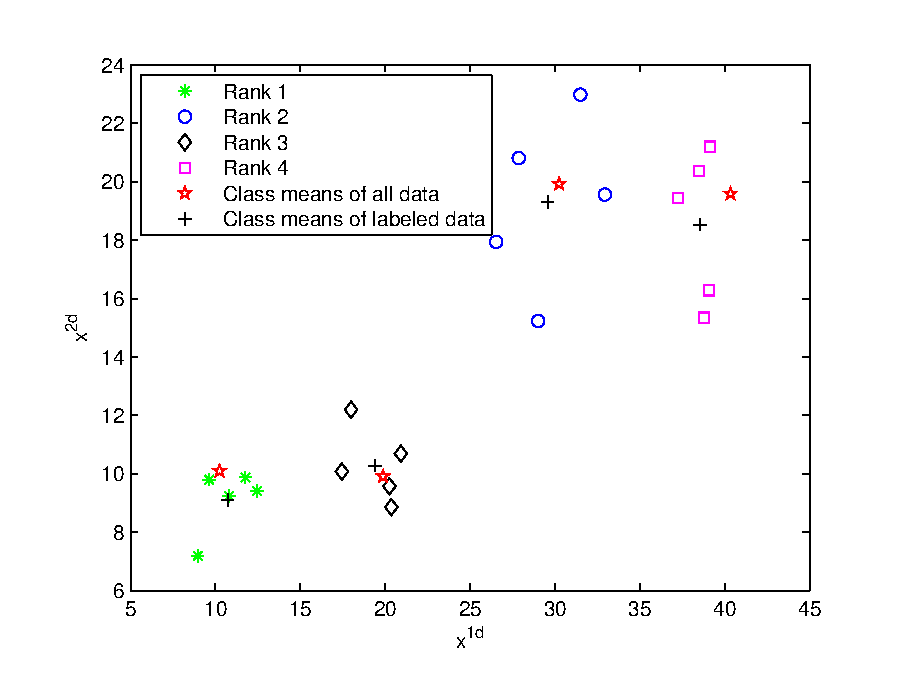
\includegraphics[width=3in]{figures/syn_labeled3}%
\label{syn_labeled}}
\hfil
\subfloat[加权策略估计的类中心情况]{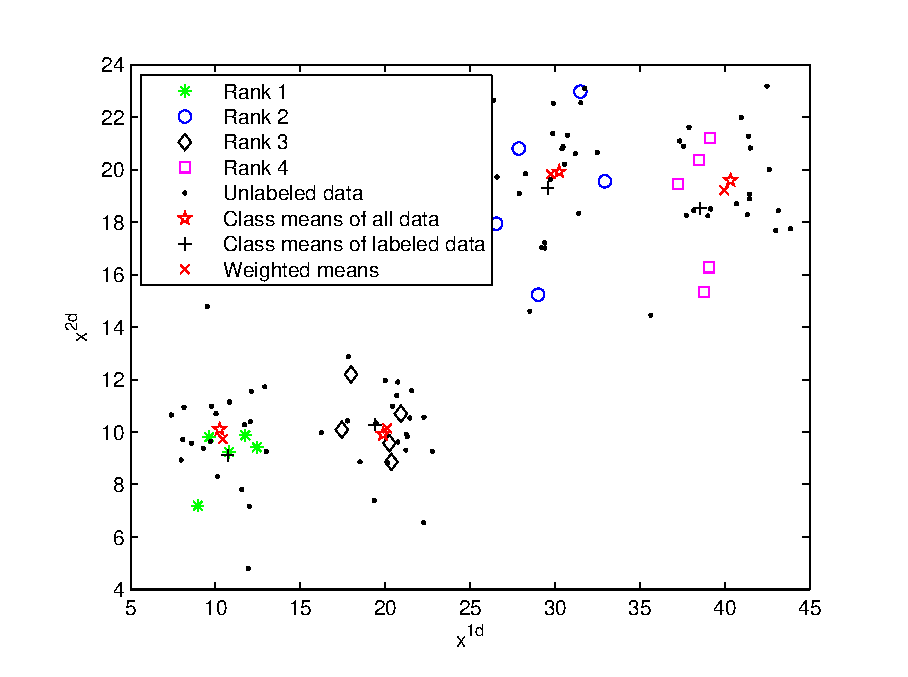
\includegraphics[width=3in]{figures/syn_weightedMeans3}%
\label{syn_weightedMeans}}
\hfil
\subfloat[KDLOR算法的投影结果]{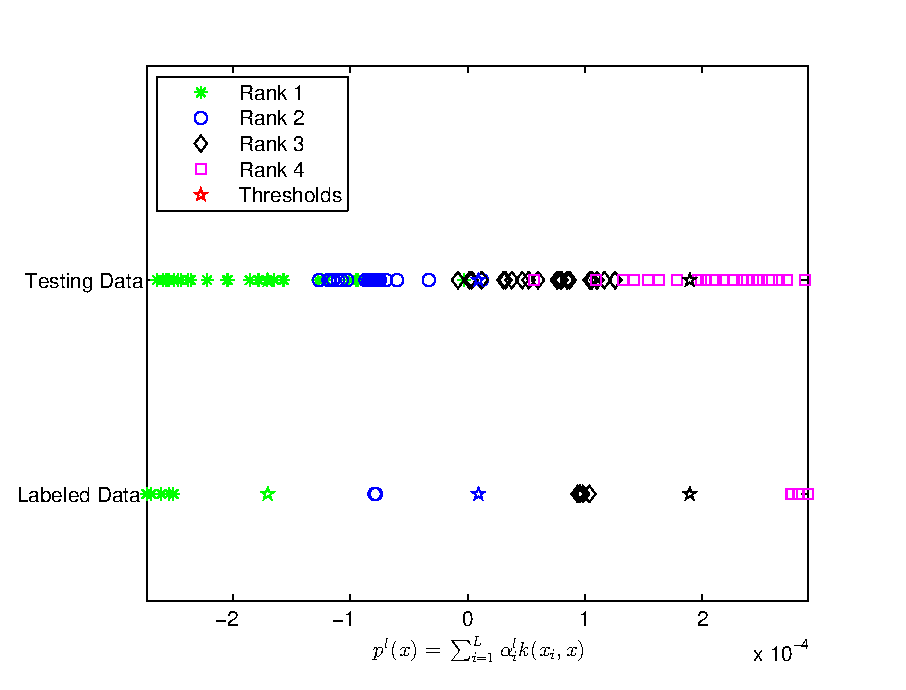
\includegraphics[width=3in]{figures/kdlor_proj3}%
\label{kdlor_proj}}
\hfil
\subfloat[WKFDOR算法的投影结果]{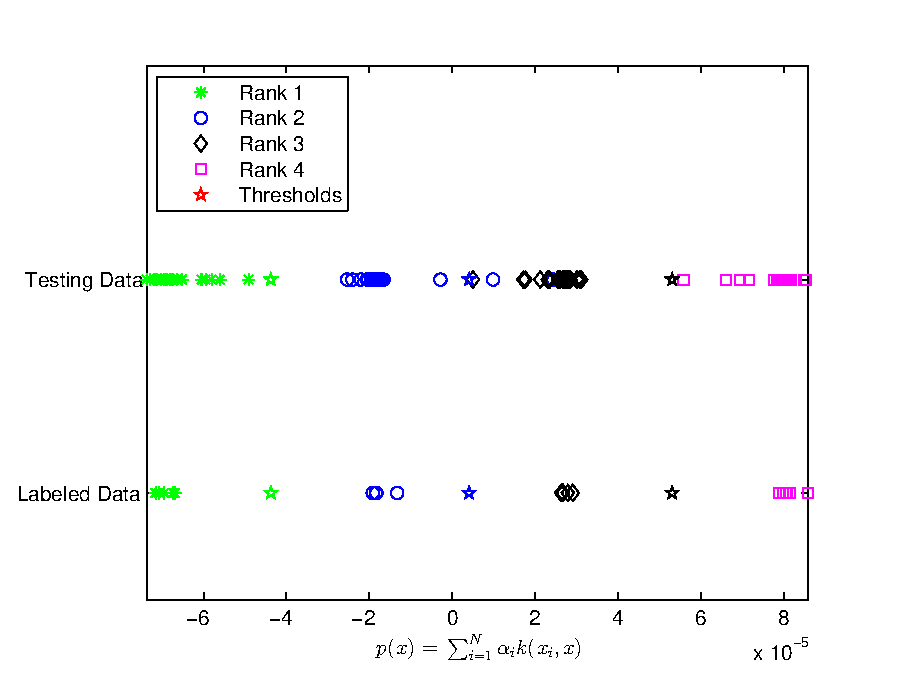
\includegraphics[width=3in]{figures/wkfdor_proj3}%
\label{wkfdor_proj}}}
\caption{合成数据集的数据分布情况和投影结果。$x^{1d}$ 和 $x^{2d}$ 分别对应样例的两个属性;$p^{l}(x)$是KDLOR算法的投影函数,其中$\alpha_{i}^{l}$是第$i$个有标签样例的系数。}
\label{syn_data}
\end{figure*}

\subsection{真实数据集}
\label{wkfdor_realData}

\begin{table}[!htbp]
\caption{真实数据集}
\label{table_realSets}
\centering
\begin{tabular}{l|cccc}
\toprule
Datasets & \# Attributes & \# Ranks & \# Training & \# Testing\\
\midrule
TAE & 5 & 3 & 100 & 51\\
Thyroid-new & 5 & 3 & 130 & 85\\
Balance & 4 & 3 & 400 & 225\\
Car & 6 & 4 & 160 & 100\\
SWD & 10 & 4 & 600 & 400\\
LEV & 4 & 5 & 600 & 400\\
ESL & 4 & 9 & 300 & 188\\
ERA & 4 & 9 & 600 & 400\\
Connect-4 & 42 & 3 & 7000 & 3000\\
\bottomrule
\end{tabular}
\end{table}

% 可以详细描述一下数据集
在这一小节中,我们使用10个真实的有序数据集(见\autoref{table_realSets})来比较WKFDOR算法和KDLOR算法。TAE、Thyroid-new、Balance、Car、Connect-4取自UCI机器学习库(UCI machine learning repository)\footnote{Car和Connect-4分别从原始数据集随机抽取一部分样例用于本实验。}\citep{Bache+Lichman:2013}。
%[M. Lichman, “UCI machine learning repository,” 2013. [Online]. Available: http://archive.ics.uci.edu/ml]。
SWD、LEV、ESL、ERA是真实的人类决策数据集,其中属性和标签都是有序值\citep{ben2006generating}。
%[A. Ben-David and L. Sterling, “Generating rules from examples of human multiattribute decision making should be simple,” Expert Systems with Applications, vol. 31, no. 2, pp. 390–396, 2006.]。

对于每个数据集,取一半的训练数据作为有标签数据,剩下的一半作为无标签数据。分别将WKFDOR算法和KDLOR算法在每个数据集上跑20遍,统计MAE和MZE的平均值和标准差。具体结果见\autoref{table_realResults20m}。

%记得加上统计测试的结果*
\begin{table*}[htbp]
\caption{KDLOR和WKFDOR在真实数据集上的测试结果。该结果是由运行20次的均值和方差组成,包括MAE和MZE两个指标。每组数据集的最优均值用粗体来表示。用秩和检验(Wilcoxon rank-sum test)做统计测试,其中显著性水平设为0.05,表中显著优于KDLOR的结果用$*$号来标记。}
\label{table_realResults20m}
\centering
\begin{tabular}{l|cc|cc}
\toprule
 & \multicolumn {2}{c|}{MAE} & \multicolumn {2}{c}{MZE} \\
 \cmidrule {2-5}
Datasets & KDLOR & WKFDOR & KDLOR & WKFDOR\\
\midrule
TAE &  {\bf 0.5402$\pm$0.0746} &  0.5471$\pm$0.0648 & 0.5392$\pm$0.0743 & {\bf 0.5353$\pm$0.0630} \\
Thyroid-new & 0.2788$\pm$0.0717 &  {\bf 0.2182$\pm$0.0576} & 0.2741$\pm$0.0736 & {\bf 0.2100$\pm$0.0619} \\
Balance & 0.4829$\pm$0.0427 &  {\bf 0.3109$\pm$0.0244}$^{*}$ & 0.4829$\pm$0.0427 & {\bf 0.3107$\pm$0.0244}$^{*}$ \\
Car & 0.3170$\pm$0.0546 &  {\bf 0.2760$\pm$0.0672} & 0.3070$\pm$0.0517 & {\bf 0.2740$\pm$0.0657} \\
SWD & {\bf 0.5740$\pm$0.0403} &  0.5833$\pm$0.0155 & 0.5097$\pm$0.0341 & {\bf 0.5060$\pm$0.0099} \\
LEV & {\bf 0.6447$\pm$0.0311} &  0.6570$\pm$0.0454 & 0.5307$\pm$0.0235 & {\bf 0.5142$\pm$0.0300} \\
ESL & {\bf 0.4415$\pm$0.0428} &  0.4660$\pm$0.0501 & {\bf 0.4436$\pm$0.0370} & 0.4553$\pm$0.0459 \\
ERA & 1.7706$\pm$0.1889 &  {\bf 1.7005$\pm$0.1524} & 0.8015$\pm$0.0256 & {\bf 0.7891$\pm$0.0238} \\
Connect-4 & 0.4982$\pm$0.0087 & {\bf 0.4828$\pm$0.0112}$^{*}$ & 0.4505$\pm$0.0094 & {\bf 0.3752$\pm$0.0097}$^{*}$ \\
%Connect-4 & 0.498183$\pm$0.008699 & 0.482817$\pm$0.011204 & 0.450467$\pm$0.009402 & 0.375200$\pm$0.009743 \\
\bottomrule
\end{tabular}
\end{table*}

MAE指标中,WKFDOR算法在5个数据集上结果的均值要优于KDLOR算法,其中在两个数据集上(Balance和Connect-4)显著优于KDLOR算法。MZE指标中,WKFDOR算法在8个数据集上结果的均值优于KDLOR算法,并在Balance和Connect-4数据集上显著优于KDLOR算法。整体来看,WKFDOR算法在处理序回归问题时具有更优的性能,尤其是MZE指标。

在真实的序回归问题中,有标签数据缺乏往往导致学习器训练不够,从而在遇到新的测试数据时不能正确地进行预测。WKFDOR算法通过加权策略利用无标签数据来更准确地估计类分布,从而获得更优的泛化性能。该实验中,WKFDOR算法得到的MZE结果几乎都优于KDLOR算法,而在一些数据集上的MAE结果没有体现出优越性,原因可能是\textit{mConsistency}算法对这些数据集中无标签数据属于每个类别的权重估计得不够准确。\textit{mConsistency}算法没有考虑数据的序关系,更偏向于以准确率为目标进行信息传播。例如,有一个真实序为3的点,它到序为1和4的类的距离相同,算法可能会得到该点以相同的置信度属于类别1和4。而在序回归问题中,如果预测该点属于类别4的置信度大于属于类别1的置信度将更有建设性,因为将其预测为4的代价通常会小于预测为1的代价(即MAE所追求的差值最小)。因此,我们将在后面的章节中提出改进的算法,使其在计算权重时考虑序信息并且估计得更加准确,从而提升性能。

\section{小结}
本章我们首先介绍了半监督序回归问题的形式化定义,和有监督序回归问题类似,半监督序回归问题的不同之处在于考虑同时使用有标签数据和无标签数据来训练模型。根据对半监督序回归问题和已有主流有监督序回归技术的分析,我们提出了一种半监督序回归技术——WKFDOR算法。该算法的主要思想是利用无标签数据来更准确地估计类的分布信息,从而获得更优的性能。通过在合成数据集和真实序回归数据集上的实验,我们验证了WKFDOR算法的有效性。









  \chapter{基于演化算法的半监督序回归技术}
\label{chap:essor}
根据前面对序回归问题的介绍可知,序回归问题中的无标签数据相比较于传统的分类问题缺失了更多的信息,所以如何利用这些无标签数据的挑战更大。上一章介绍了我们提出的基于加权核判别分析的半监督序回归技术(WKFDOR),它通过计算无标签数据的隶属度和加权策略来利用无标签数据,从而更准确地估计类分布。因为WKFDOR算法中使用的权重是否准确将会对学习性能产生重要的影响,所以这一章节中我们将对\autoref{alg_mem}得到的权重进行优化,从而改进WKFDOR算法的性能。优化权重主要通过结合序信息来更准确地估计权重。一方面,这样能够更充分地使用序回归问题的数据信息;另一方面,引入序信息能够更准确地估计权重,最终提升学习性能。
%序回归问题中,同时引入无标签数据和序信息往往使得问题非凸不可导
%To further improve the overall performance, an evolutionary algorithm (i.e., differential evolution) is employed to evolve the weights.

然而,当权重作为\autoref{wkfdor}中的优化变量时,该优化问题是一个非凸且不可导的问题。在\autoref{chap:review}中,我们分析了演化算法在处理这类问题中的优势。所以,我们使用演化算法来改善权重,提出了一种基于演化算法的半监督序回归技术。

在本章中,我们将首先提出基于演化算法的半监督核判别分析序回归算法(evolutionary semi-supervised ordinal regression using weighted kernel Fisher discriminant analysis, ESSOR)。其次,我们将通过实验来验证演化算法在进一步提升学习性能上的有效性。本章还将介绍在处理大规模数据集上的加速方法。

%然而,当权重作为\autoref{wkfdor}中的优化变量时,该优化问题是一个非凸且不可导的问题。传统的优化算法(例如梯度下降算法)难以处理这种类型的问题,而演化算法(evolutionary algorithm, EA)适用于处理。所以,在这一章中我们使用了演化算法来改善权重,具体的说是差分进化(differential evolution, DE)算法[R. Storn and K. Price, “Differential evolution–a simple and effi- cient heuristic for global optimization over continuous spaces,” Journal of Global Optimization, vol. 11, no. 4, pp. 341–359, 1997.]。差分进化算法是一种高效的处理连续优化问题的演化算法,它简单易用,并且容易并行化。此外,差分进化算法具有收敛好和实现快的属性[K. Price, R. M. Storn, and J. A. Lampinen, Differential Evolu- tion: A Practical Approach to Global Optimization. Secaucus, NJ, USA: Springer-Verlag New York, Inc., 2005.]。因此,我们采用差分进化算法。下面我们首先介绍个体表示(individual representation)方法,即如何表示我们需要优化的变量;其次我们介绍适应度评估函数(fitness function),最后介绍我们提出的基于演化算法的半监督核判别分析序回归算法(evolutionary semi-supervised ordinal regression using weighted kernel Fisher discriminant analysis, ESSOR)。

% \section{演化算法及演化机器学习}
% 在人工智能领域,演化算法(EA)是演化计算的一个子集,是一类基于种群的元启发式优化算法。用种群中的个体来表示优化问题中的候选解,而适应度函数(fitness function)用于决定个体的质量。EA使用类似于生物进化的机制,例如交叉、变异、选择等来实现种群的进化,最终得到满足一定条件的优化问题的解。\autoref{alg_EA}给出了演化算法的基本框架。其中,终止条件一般是代数达到预设的最大代数,或者是计算时间达到限制,或者是适应度达到一定的标准。

% \IncMargin{1em}
% \begin{algorithm}
% \SetKwData{Left}{left}\SetKwData{This}{this}\SetKwData{Up}{up}
% \SetKwFunction{Union}{Union}\SetKwFunction{FindCompress}{FindCompress}
% \SetKwInOut{Input}{input}\SetKwInOut{Output}{output}
% \emph{初始化种群$P(0) = \{x_{1},x_{2},\dots ,x_{N_{p}}\}$}\;
% \emph{令代数计数器$g = 0$}\;
% \emph{评估$P(0)$中每个个体的适应度}\;
% \Repeat{满足EA的终止条件}{
%     \emph{通过交叉、变异、选择等算子,由$P(g)$生成新的种群$P(g+1)$}\;
%     \emph{评估$P(g)$中每个个体的适应度}\;
%     \emph{$g=g+1$}\;
% }
% \caption{演化算法的基本框架}\label{alg_EA}
% \end{algorithm}\DecMargin{1em}

% 优化算法通常可以分为三类:解析法(calculus-based)、枚举法(enumerative)和随机法\citep{潘正君1998演化计算}。解析法在求解过程中需要使用目标函数的解析性质,例如一阶导数、二阶导数等。通常,解析法根据目标函数的梯度信息来确定下一步的搜索方向,如Newton法、共轭梯度下降法等。此外,解析法在求解非凸问题时,往往会根据最陡的方向找到一个局部最优点,而难以找到一个全局最优解。枚举法是一种暴力搜索的方法,它不使用启发信息,而直接对候选的解空间进行逐一枚举计算。对于大规模的优化问题,枚举法速度慢,难以适用。演化算法属于随机法的一种,它使用随机性的转移规则而不是确定性的转移规则,因而能跳出局部最优,搜索到全局较优的解。相比较于解析法,演化算法不需要目标的解析性质,因此它能够处理目标函数不可导的优化问题。此外,相比较于枚举法,演化算法是一种元启发式算法,它能够通过适应度函数和进化算子引导种群的进化,以较快地速度找到全局较优的解。

% EA在求解各种优化问题时,通常都能得到不错的近似解,因为它没有对潜在的适应度曲面做任何假设。尤其是在求解一些非凸、目标函数不可导、甚至连优化目标都难以形式化定义的优化问题时,演化算法具有明显的优势。

%可以把这一小节放到上面去。
%In this circumstance, evolutionary algorithms (EA) are ac- claimed, since they perform well for this type of problems. Recently, EA have been used in many machine learning problems, such as feature extraction [13], pattern recognition [14] and ensemble learning [15].

\section{基于演化算法的半监督核判别分析序回归算法}
%当权重作为\autoref{wkfdor}中的优化变量时,该优化问题是一个非凸且不可导的问题。传统的优化算法(例如梯度下降算法)难以处理这种类型的问题,而演化算法(evolutionary algorithm, EA)适用于处理。
根据前面的分析可知,我们需要借助演化算法来优化权重,进而提升WKFDOR算法的性能。本节我们基于WKFDOR提出改进的算法——ESSOR。下面我们首先介绍个体表示方法,即如何表示我们需要优化的变量;其次介绍适应度评估函数;最后根据问题特点,我们选择了一种处理连续优化问题的演化算法——差分进化算法(differential evolution, DE),并给出了ESSOR的算法步骤。

\subsection{个体表示}
最简单直接的方法就是将整个无标签数据的权重矩阵作为一个个体,但是这样的话每个个体的维度将是\((N-L)\times K\)(注意,有标签数据的权重是固定的,我们只需要去优化无标签数据的权重),即和无标签数据量成正比。可以想象,当我们使用大量的无标签数据时,每个个体的维度将非常高,这对演化算法来说无疑是个灾难。因此,我们提出了一个新颖的个体表示方法,它能够将个体大小减小到\(K\)(即序的个数)。

个体的作用是用来表示解空间,使得优化算法能够不断地在适应度函数的引导下在解空间产生更优的个体。在该问题中,我们需要不断更新权重,而新的权重可以用已有的权重通过一定的规则产生。因此,我们考虑将更新权重规则参数化,通过控制这些参数来间接引导权重的更新。我们给第\(k\)个类别引入一个参数\(\lambda_{k}\),并将个体定义为\(\lambda=(\lambda_{1},\lambda_{2},\dots,\lambda_{K})\)。新的权重通过下面的更新规则产生:
\begin{equation}
\label{mem_updateRule}
u_{jk}^{'}=\frac{u_{jk}^{\lambda_{k}}}{\Sigma_{k=1}^{K} u_{jk}^{\lambda_{k}}}
\end{equation}
其中 \(u_{jk}\)是\autoref{alg_mem}估计的权重,将其作为初始权重。新的 \(\mathcal{M}_{k}\) 和 \(\mathcal{N}\)可以通过\autoref{M}和\autoref{N}计算得到,新的投影向量\(w\) 可以通过求解\autoref{wkfdor}的优化问题得到。根据上面的分析,\(\lambda\)引导了无标签数据权重的更新,从而将原问题转化成了搜索最优的\(\lambda\)。注意,有标签数据的权重(即直接从它们的标签可获得)在演化过程中固定不变。

我们对权重更新规则\autoref{mem_updateRule}进行了一定的数学分析,下面的这些特性保证了它能够合理地调整权重:
\begin{enumerate}
\item[1.]对每一个数据点,权重更新规则能够改变它属于两个不同类别的权重的相对值。
\\ \[ \frac{u_{jk_{1}}^{'}}{u_{jk_{2}}^{'}}=\frac{u_{jk_{1}}^{\lambda_{k_{1}}}}{u_{jk_{2}}^{\lambda_{k_{2}}}} \neq \frac{u_{jk_{1}}}{u_{jk_{2}}} \]
%
\item[2.]对两个不同的数据点,权重更新规则能够改变它们属于同一个类别的权重的相对值。
\\ \[ \frac{u_{ik}^{'}}{u_{jk}^{'}}=\frac{u_{ik}^{\lambda_{k}} \sum_{k=1}^{K}u_{jk}^{\lambda_{k}}}{u_{jk}^{\lambda_{k}} \sum_{k=1}^{K}u_{ik}^{\lambda_{k}}} \neq \frac{u_{ik}}{u_{jk}} \]
%
\item[3.]权重的改变不仅和\(\lambda\)相关,同时也受到初始权重的影响。
\\ \[ \frac{u_{ik}^{'}}{u_{ik}}=\frac{u_{ik}^{\lambda_{k}-1}}{\Sigma_{k=1}^{K} u_{ik}^{\lambda_{k}}} \]
\end{enumerate}
为了进一步观察权重更新规则的特性,假设\(\lambda_{k}\)随机取值于一个\([0,2]\)范围内的均匀分布,\autoref{fig_expFunc}画出了一组以不同\(u\)值为底数的指数函数。
\begin{figure}[h]
   \centering
   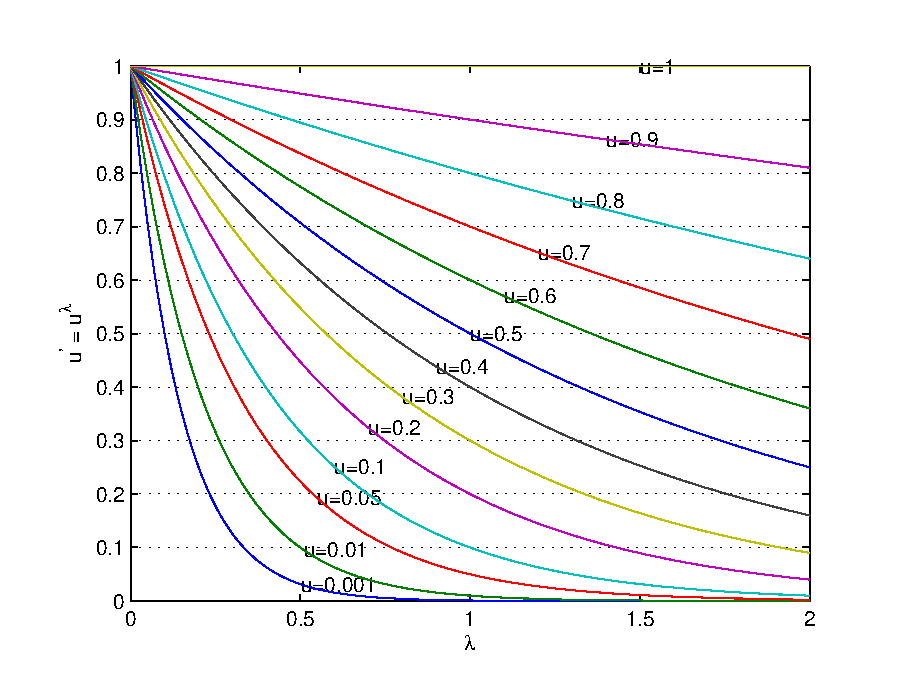
\includegraphics[width=4.5in]{figures/expfunc}
\caption{以不同\(u\)值为底数的指数函数}
\label{fig_expFunc}
\end{figure}
%
通过\autoref{fig_expFunc}中不同曲线的形状可以看出,当初始权重有相对比较极端的值时(即接近\(1\)或\(0\)的数值,表示该无标签数据点有很大的置信度属于或不属于相应的类别),它将有相对更大的概率保持在初始值附近。权重更新规则的这个特性体现了其在一定程度上相信初始权重值,所以这个演化过程可以看作是对初始权重的一种微调。

\subsection{适应度函数}
通常,演化过程是由一个适应度评估函数来驱动的。这一节中,我们定义了算法使用的适应度函数,它是由以下三个指标以递减的优先级组合而成:
\begin{enumerate}
\item[1.]在有标签数据上对算法进行评估得到的MAE;
\item[2.]在有标签数据上对算法进行评估得到的MZE;
\item[3.]\autoref{wkfdor}优化问题的目标函数最优值,将其命名为 \textit{ORfval}。
\end{enumerate}
该适应度函数不计算确切的适应度值,而是通过这三个指标来比较两个个体以决定哪个个体适应度更高,其具体实现见\autoref{alg_fitness}。

\IncMargin{1em}
\begin{algorithm}
\SetKwData{Left}{left}\SetKwData{This}{this}\SetKwData{Up}{up}
\SetKwFunction{Union}{Union}\SetKwFunction{FindCompress}{FindCompress}
\SetKwInOut{Input}{input}\SetKwInOut{Output}{output}
\Input{个体 $\lambda^{a}$的$(MAE_{\lambda^{a}},MZE_{\lambda^{a}},ORfval_{\lambda^{a}})$;\\
个体$\lambda^{b}$的$(MAE_{\lambda^{b}},MZE_{\lambda^{b}},ORfval_{\lambda^{b}})$}
\Output{$\lambda^{a}$和$\lambda^{b}$的适应度比较结果}
\BlankLine
\emph{$num\_priorities = 3$}\;
\For{$i=1$ \KwTo $num\_priorities$}{
\emph{$metric_{\lambda^{a}} \gets$ $\lambda^{a}$第$i$优先级的指标}\;
\emph{$metric_{\lambda^{b}} \gets$ $\lambda^{b}$第$i$优先级的指标}\;

\uIf{$metric_{\lambda^{a}} < metric_{\lambda^{b}}$}{
\emph{$fitness(\lambda^{a}) > fitness(\lambda^{b})$}\;
\emph{\textbf{break}}\;
}

\uElseIf{$metric_{\lambda^{a}} > metric_{\lambda^{b}}$}{
\emph{ $fitness(\lambda^{a}) < fitness(\lambda^{b})$}\;
\emph{\textbf{break}}\;
}

\Else{
\emph{$fitness(\lambda^{a}) == fitness(\lambda^{b})$}\;
}

}
\caption{适应度评估函数}\label{alg_fitness}
\end{algorithm}\DecMargin{1em}

通常,将在验证集(validation dataset)上的分类准确率作为适应度度量。但是,在半监督学习问题中有标签数据量很少,如果从中取出一部分用来作验证集的话将会增加学习难度并很有可能导致更差的学习性能。 因此,这里我们在有标签数据集上评估算法的MAE和MZE。在序回归问题中,我们希望预测的标签能够和实际标签尽可能相近,所以MAE比MZE更能体现算法的性能,因此这里我们给MAE更高的优先级。前两个指标用来最小化序回归学习器的经验风险(empirical risk),使其能够获得基本的识别能力。但是仅在一个小的有标签数据集上最小化分类误差很可能导致模型过拟合(over-fitting),所以这里我们还将在整个训练集上计算到的ORfval引入进来。ORfval用来最小化预测风险,它能够促进同类别的数据点更加紧凑而相邻类的数据点能够更加分散(在映射后的空间里)。总的来说,在有标签数据集上评估的MAE和MZE指示了模型已经学习正确的程度,而ORfval在概念上类似于指示学习器的潜能并用来防止过拟合\citep{liu2000evolutionary}\citep{liu2003evolutionary}。
%[C. Liu and H. Wechsler, “Evolutionary pursuit and its applica- tion to face recognition,” IEEE Transactions on Pattern Analysis and Machine Intelligence, vol. 22, no. 6, pp. 570–582, 2000.]
%[H. Liu and S.-T. Huang, “Evolutionary semi-supervised fuzzy clustering,” Pattern Recognition Letters, vol. 24, no. 16, pp. 3105–3113, 2003.]。
因此,由\autoref{alg_fitness}的适应度函数所驱动的演化过程可以达到良好的学习性能和泛化能力。

\subsection{差分进化}

我们选择差分进化(differential evolution, DE)算法\citep{storn1995differential}来优化参数向量\(\lambda\),由此来间接获得微调的权重。差分进化算法是由Storn和Price在1995年提出\citep{storn1995differential},当时是为了处理Chebychev问题。与传统的演化算法不同,DE从当前种群获得距离和方向信息用以指导搜索方向。这主要体现在差分进化的变异步长受当前种群的个体间差异影响,而在遗传算法、演化策略等演化算法中变异步长以相同的概率分布函数抽样。

\begin{equation}
\label{DE_mutation}
u_{i}(g) = x_{i_{1}}(g)+\beta(x_{i_{2}}(g)-x_{i_{3}}(g))
\end{equation}

\begin{equation}
\label{DE_crossover}
x^{'}_{ij}(g)=
\begin{cases}
u_{ij}(g)& j \in J \\
x_{ij}(g)& \text{其他情况}
\end{cases}
\end{equation}

在差分进化算法中,通过变异、交叉、选择三种算子来产生新的种群。
\begin{enumerate}
\item[1.变异:]\autoref{DE_mutation}给出了差分进化的变异算子。对于每一个父代个体\(x_{i}(g)\),通过该变异算子产生测试向量\(u_{i}(g)\)。其中,\(x_{i_{1}}(g)\)、\(x_{i_{2}}(g)\)、\(x_{i_{3}}(g)\)是从第\(g\)代种群中随机选择的个体,且\(i \neq i_{1} \neq i_{2} \neq i_{3}\)。比例因子\(\beta > 0\),用来控制差分变量的放大程度。

\item[2.交叉:]通过父代个体\(x_{i}(g)\)与测试个体\(u_{i}(g)\)的离散重组产生子代个体\(x^{'}_{i}(g)\),\autoref{DE_crossover}给出了差分进化的交叉算子。其中,\(x_{ij}(g)\)表示\(x_{i}(g)\)的第\(j\)个元素,\(J\)是交叉位的集合。常见的交叉方式有二项式交叉和指数交叉,\autoref{alg_DE_crossover}给出了二项式交叉方式生成交叉位集合的算法,其中\(p_{r}\)是重组概率。

\item[3.选择:]对每个个体进行适应度评估,如果子代个体的适应度优于其父代个体,则用子代替换其父代;否则父代个体继续存活至下一代。

\end{enumerate}

%二项式交叉
\IncMargin{1em}
\begin{algorithm}
\SetKwData{Left}{left}\SetKwData{This}{this}\SetKwData{Up}{up}
\SetKwFunction{Union}{Union}\SetKwFunction{FindCompress}{FindCompress}
\SetKwInOut{Input}{input}\SetKwInOut{Output}{output}
\Input{问题维度$n_{x}$}
\Output{交叉位集合$J$}
\emph{$j^{*}\sim U \left( 1,n_{x} \right)$}\;
\emph{$J = \{j^{*}\}$}\;
\For{$j = 1$ \KwTo $n_{x}$}{
    \If{$U(0,1)<p_{r}$且$j\neq j^{*}$}{
        \emph{$J=J\cup \{j\}$}\;
    }
}
\caption{二项式交叉方式生成交叉位集合算法}\label{alg_DE_crossover}
\end{algorithm}\DecMargin{1em}

%差分进化算法
\IncMargin{1em}
\begin{algorithm}
\SetKwData{Left}{left}\SetKwData{This}{this}\SetKwData{Up}{up}
\SetKwFunction{Union}{Union}\SetKwFunction{FindCompress}{FindCompress}
\SetKwInOut{Input}{input}\SetKwInOut{Output}{output}
\emph{初始化种群大小$NP$、比例因子$\beta$和重组概率$p_{r}$}\;
\emph{$g=0$}\;
\emph{初始化初代种群$P(0)$}\;
        \Repeat{满足DE的停止准则}{
            \For{每个个体$x_{i}(g) \in P(g)$}{
                \emph{用变异算子产生测试个体$u_{i}(g)$}\;
                \emph{用交叉算子产生子代个体$x^{'}_{i}(g)$}\;
                \emph{评估$x_{i}(g)$和$x^{'}_{i}(g)$的适应度}\;
                \eIf{$f(x^{'}_{i}(g))$优于$f(x_{i}(g))$}{
                    \emph{将$x^{'}_{i}(g)$加入$P(g+1)$}\;
                }{
                    \emph{将$x_{i}(g)$加入$P(g+1)$}\;
                }
}
        \emph{$g=g+1$}\;
}
\emph{返回适应度最好的个体}\;
\caption{差分进化算法}\label{alg_DE}
\end{algorithm}\DecMargin{1em}
% 详细介绍差分进化算法
%[R. Storn and K. Price, “Differential evolution–a simple and effi- cient heuristic for global optimization over continuous spaces,” Journal of Global Optimization, vol. 11, no. 4, pp. 341–359, 1997.]。

\autoref{alg_DE}给出了一般差分进化算法的步骤。差分进化是一种高效的处理连续优化问题的演化算法,简单易用,并且容易并行化。此外,差分进化算法还具有收敛好和实现快的特点\citep{price2006differential}。
%[K. Price, R. M. Storn, and J. A. Lampinen, Differential Evolu- tion: A Practical Approach to Global Optimization. Secaucus, NJ, USA: Springer-Verlag New York, Inc., 2005.]。
因此,我们采用差分进化算法来搜索最优的\(\lambda\)。在初代种群中引入一个个体\(\lambda=(1,1,\dots,1)\),用来表示初始权重。初代种群的其它个体将在一个给定范围内随机生成。基于上面的介绍和分析,我们在\autoref{alg_ESSOR}提出了基于演化算法的半监督序回归算法——ESSOR。其中,\(\lambda_{g}^{t}\)是通过DE的交叉和变异算子产生的新的个体,用于探索解空间。分别将\(\lambda_{g}\)和\(\lambda_g^{t}\)代入\autoref{mem_updateRule}的权重更新规则,得到新的权重矩阵\((u_{jk}^{'})_{N \times K}\)和\((u_{jk}^{t})_{N \times K}\)。再分别将两个新的权重矩阵应用到WKFDOR算法得到半监督序回归模型(ORfval可以同时得到)。在有标签数据集上评估得到的半监督序回归模型,得到相应的MAE和MZE。结合ORfval,得到适应度的三元组。由\autoref{alg_fitness}得到适应度评价结果,根据结果决定保留子代个体还是父代个体至下一代种群。
%权重更新规则见\autoref{mem_updateRule},适应度函数见\autoref{alg_fitness}。
其中,DE的停止准则是迭代次数(maximum generation)达到预设的最大代数。从最后的种群中选出最优的个体,即最优的\(\lambda\)。根据权重更新规则得到最优的权重矩阵,并应用WKFDOR算法得到最终的序回归模型。

%可以将得到fitness的过程写成算法

\IncMargin{1em}
\begin{algorithm}
\SetKwData{Left}{left}\SetKwData{This}{this}\SetKwData{Up}{up}
\SetKwFunction{Union}{Union}\SetKwFunction{FindCompress}{FindCompress}
\SetKwInOut{Input}{input}\SetKwInOut{Output}{output}
\Input{有标签数据$(X^{l},Y^{l})=\{(x_{1:L},y_{1:L})\}$;\\
无标签数据$X^{u}=\{(x_{L+1:N})\}$}
\Output{序回归学习器}
\emph{初始权重$(u_{jk})_{N \times K}$ $\leftarrow$ \textit{mConsistency}算法}\;
\emph{初始化初代种群}\;
        \Repeat{满足DE的停止准则}{
            \For{第$g$代种群的每个个体$\lambda$}{
                \emph{$\lambda_{g}^{t}$ $\leftarrow$ 交叉和变异算子, $\lambda_{g}$}\;
                \emph{$(u_{jk}^{'})_{N \times K}$ $\leftarrow$ 权重更新规则, $(u_{jk})_{N \times K}$, $\lambda_{g}$}\;
                \emph{$(u_{jk}^{t})_{N \times K}$ $\leftarrow$ 权重更新规则, $(u_{jk})_{N \times K}$, $\lambda_{g}^{t}$}\;
                \emph{$fitness(\lambda_{g})$ $\leftarrow$ WKFDOR, $(X^{l},Y^{l})$, $(u_{jk}^{'})_{N \times K}$}\;
                \emph{$fitness(\lambda_{g}^{t})$ $\leftarrow$ WKFDOR, $(X^{l},Y^{l})$, $(u_{jk}^{t})_{N \times K}$}\;
                \eIf{$fitness(\lambda_{g}^{t}) > fitness(\lambda_{g})$}{
                    \emph{$\lambda_{g+1}=\lambda_{g}^{t}$}\;
                }{
                    \emph{$\lambda_{g+1}=\lambda_{g}$}\;
                }
}
        \emph{$g=g+1$}\;
}
\emph{从末代种群中选出最优的个体$\lambda^{*}$}\;
\emph{$(u_{jk}^{*})_{N \times K}$ $\leftarrow$ 权重更新规则, $(u_{jk})_{N \times K}$, $\lambda^{*}$}\;
\emph{最终的序回归学习器 $\leftarrow$ WKFDOR, $(u_{jk}^{*})_{N \times K}$}\;
\caption{ESSOR}\label{alg_ESSOR}
\end{algorithm}\DecMargin{1em}

\section{实验验证}
ESSOR算法是在WKFDOR算法基础上做了改进,它基于演化算法去优化无标签数据属于每个类别的权重,使学习器最终拥有更好的泛化性能。 我们在这一节通过实验来验证ESSOR算法的性能,具体的做法是在\autoref{table_realSets}列出的数据集上比较KDLOR、WKFDOR、ESSOR三个算法的性能。

\subsection{实验设置}
对于KDLOR算法和WKFDOR算法,采用和\autoref{wkfdor_expSet}相同的实验设置。对于ESSOR算法,我们也使用和KDLOR、WKFDOR相同的\(\mu\)、\(C\) 和 \(\sigma\) ,并使用和WKFDOR相同的 \(\alpha\) 和\(\varepsilon\)(\textit{mConsistency}算法中的参数)。对于演化部分,我们将DE中的参数设置如下:\(NP = 10 \times K\);\(\beta = 0.85\);\(p_{r} = 0.9\);\(\lambda_{k} \in [0,2]\);\(maximum\_generation = 300\)。

%\(population\;size = 10 \times K\);\(scale\;factor = 0.85\);\(crossover\;rate=0.9\);\(\lambda_{k} \in [0,2]\);\(maximum\;generation = 300\)。

和\autoref{wkfdor_realData}中的做法相同,对于每个数据集,取一半的训练数据作为有标签数据,剩下的一半作为无标签数据。

\subsection{处理大数据}

%写抽样做的算法
\IncMargin{1em}
\begin{algorithm}
\SetKwData{Left}{left}\SetKwData{This}{this}\SetKwData{Up}{up}
\SetKwFunction{Union}{Union}\SetKwFunction{FindCompress}{FindCompress}
\SetKwInOut{Input}{input}\SetKwInOut{Output}{output}
\Input{有标签数据$(X^{l},Y^{l})=\{(x_{1:L},y_{1:L})\}$;\\
无标签数据$X^{u}=\{(x_{L+1:N})\}$}
\Output{序回归学习器}
\emph{初始权重$(u_{jk})_{N \times K}$ $\leftarrow$ \textit{mConsistency}算法}\;
\emph{从$(X^{l},Y^{l})$中随机抽取sampling\_size个样例作为采样的有标签数据$(X_{s}^{l},Y_{s}^{l})$}\;
\emph{从$X^{u}$中随机抽取sampling\_size个样例作为采样的无标签数据$X_{s}^{u}$}\;
\emph{从$(u_{jk})_{N \times K}$抽取相应的采样的初始权重矩阵$(u_{jk})_{N \times K}^{s}$}\;
\emph{初始化初代种群}\;
        \Repeat{满足DE的停止准则}{
            \For{第$g$代种群的每个个体$\lambda$}{
                \emph{$\lambda_{g}^{t}$ $\leftarrow$ 交叉和变异算子, $\lambda_{g}$}\;
                \emph{$(u_{jk}^{'})_{N \times K}^{s}$ $\leftarrow$ 权重更新规则, $(u_{jk})_{N \times K}^{s}$, $\lambda_{g}$}\;
                \emph{$(u_{jk}^{t})_{N \times K}^{s}$ $\leftarrow$ 权重更新规则, $(u_{jk})_{N \times K}^{s}$, $\lambda_{g}^{t}$}\;
                \emph{$fitness(\lambda_{g})$ $\leftarrow$ WKFDOR, $(X_{s}^{l},Y_{s}^{l})$, $(u_{jk}^{'})_{N \times K}^{s}$}\;
                \emph{$fitness(\lambda_{g}^{t})$ $\leftarrow$ WKFDOR, $(X_{s}^{l},Y_{s}^{l})$, $(u_{jk}^{t})_{N \times K}^{s}$}\;
                \eIf{$fitness(\lambda_{g}^{t}) > fitness(\lambda_{g})$}{
                    \emph{$\lambda_{g+1}=\lambda_{g}^{t}$}\;
                }{
                    \emph{$\lambda_{g+1}=\lambda_{g}$}\;
                }
}
        \emph{$g=g+1$}\;
}
\emph{从末代种群中选出最优的个体$\lambda^{*}$}\;
\emph{$(u_{jk}^{*})_{N \times K}$ $\leftarrow$ 权重更新规则, $(u_{jk})_{N \times K}$, $\lambda^{*}$}\;
\emph{最终的序回归学习器 $\leftarrow$ WKFDOR, $(u_{jk}^{*})_{N \times K}$}\;
\caption{ESSOR-S}\label{alg_ESSOR_sampling}
\end{algorithm}\DecMargin{1em}

ESSOR使用演化算法来优化权重,而演化算法需要通过迭代来产生新的更优的个体。对于大数据集,例如\autoref{table_realSets}中的Connect-4数据集(有7000个训练样例),如果对每代种群的每个个体都使用全部训练样例来建模、评估适应度,将会使计算量变得非常大。因此,我们使用随机采样方法来降低建模和适应度评估的计算代价。具体算法见\autoref{alg_ESSOR_sampling},我们将其命名为ESSOR-Sampling,简称为ESSOR-S。步骤2—4从原来的数据集中随机抽取一部分用于在差分进化时建模和评估适应度。由于实验设置中有标签数据和无标签数据数量相同,所以我们在步骤2—3中使用相同的采样参数,并令\(sampling\_size = 300\)。

通过随机采样的方法,可以加快建模和适应度评估的计算速度,从而使DE能够在更短的时间内收敛。但是,这样做的代价是损失了一定的算法性能(MAE和MZE)。对于一个大数据集,如果我们能在较短的时间内获得一个相对不错的结果,在一些应用场景下往往更加可取。本实验中,Sushi和Connect-4数据集使用ESSOR-S算法。

\subsection{实验结果}
我们分别将KDLOR、WKFDOR和ESSOR在\autoref{table_realSets}中的每个数据集上跑20遍,统计MAE和MZE的平均值和标准差。具体结果见\autoref{table_essor_mae}和\autoref{table_essor_mze}。
%其中Connect数据集使用ESSOR-S算法
%再加一个标记,即ESSOR显著优于WKFDOR的打+号

%MAE
\begin{table*}[!htbp]
\caption{KDLOR、WKFDOR、ESSOR在真实数据集上的测试MAE,由运行20次的均值和方差组成。每组数据集的最优均值用粗体来表示。用秩和检验(Wilcoxon rank-sum test)做统计测试,其中显著性水平设为0.05,表中显著优于KDLOR的结果用$*$号来标记。}
\label{table_essor_mae}
\centering
\begin{tabular}{l|ccc}
\toprule
 & \multicolumn {3}{c}{MAE} \\
 \cmidrule {2-4}
Datasets & KDLOR & WKFDOR & ESSOR \\
\midrule
TAE &  0.5402$\pm$0.0746 &  0.5471$\pm$0.0648 & {\bf 0.5363$\pm$0.0709} \\
Thyroid-new & 0.2788$\pm$0.0717 &  0.2182$\pm$0.0576 & {\bf 0.2159$\pm$0.0613}$^{*}$ \\
Balance & 0.4829$\pm$0.0427 &  {\bf 0.3109$\pm$0.0244}$^{*}$ & 0.3227$\pm$0.0401$^{*}$ \\
Car & 0.3170$\pm$0.0546 &  0.2760$\pm$0.0672 & {\bf 0.2750$\pm$0.0622} \\
SWD & 0.5740$\pm$0.0403 &  0.5833$\pm$0.0155 & {\bf 0.5537$\pm$0.0204} \\
LEV & 0.6447$\pm$0.0311 &  0.6570$\pm$0.0454 & {\bf 0.5757$\pm$0.0330}$^{*}$ \\
ESL & 0.4415$\pm$0.0428 &  0.4660$\pm$0.0501 & {\bf 0.4293$\pm$0.0339} \\
ERA & 1.7706$\pm$0.1889 &  1.7005$\pm$0.1524 & {\bf 1.5511$\pm$0.1312}$^{*}$ \\
Sushi & 1.0210$\pm$0.0149 & 1.0132$\pm$0.0140 & {\bf 0.9815$\pm$0.0148}$^{*}$ \\
Connect-4 & 0.4982$\pm$0.0087 & 0.4828$\pm$0.0112$^{*}$ & {\bf 0.4820$\pm$0.0212}$^{*}$ \\
\bottomrule
\end{tabular}
\end{table*}

%MZE
\begin{table*}[!htbp]
\caption{KDLOR、WKFDOR、ESSOR在真实数据集上的测试MZE,由运行20次的均值和方差组成。每组数据集的最优均值用粗体来表示。用秩和检验(Wilcoxon rank-sum test)做统计测试,其中显著性水平设为0.05,表中显著优于KDLOR的结果用$*$号来标记。}
\label{table_essor_mze}
\centering
\begin{tabular}{l|ccc}
\toprule
& \multicolumn {3}{c}{MZE} \\
 \cmidrule {2-4}
Datasets & KDLOR & WKFDOR & ESSOR \\
\midrule
TAE & 0.5392$\pm$0.0743 & 0.5353$\pm$0.0630 &  {\bf 0.5294$\pm$0.0700} \\
Thyroid-new  & 0.2741$\pm$0.0736 & 0.2100$\pm$0.0619 &  {\bf 0.2071$\pm$0.0630}$^{*}$ \\
Balance & 0.4829$\pm$0.0427 & {\bf 0.3107$\pm$0.0244}$^{*}$ &  0.3184$\pm$0.0406$^{*}$ \\
Car & 0.3070$\pm$0.0517 & 0.2740$\pm$0.0657 &  {\bf 0.2730$\pm$0.0598} \\
SWD & 0.5097$\pm$0.0341 & 0.5060$\pm$0.0099 &  {\bf 0.4875$\pm$0.0131} \\
LEV & 0.5307$\pm$0.0235 & 0.5142$\pm$0.0300 &  {\bf 0.4940$\pm$0.0190}$^{*}$ \\
ESL & 0.4436$\pm$0.0370 & 0.4553$\pm$0.0459 &  {\bf 0.4032$\pm$0.0260}$^{*}$ \\
ERA  & 0.8015$\pm$0.0256 & 0.7891$\pm$0.0238 & {\bf 0.7729$\pm$0.0287} \\
Sushi & 0.7254$\pm$0.0252 & 0.7002$\pm$0.0216$^{*}$ & {\bf 0.6922$\pm$0.0067}$^{*}$ \\
Connect-4 & 0.4505$\pm$0.0094 & {\bf 0.3752$\pm$0.0097}$^{*}$ & 0.3762$\pm$0.012$^{*}$ \\
\bottomrule
\end{tabular}
\end{table*}

%\begin{table*}[htbp]
%\caption{Test results of KDLOR, WKFDOR and ESSOR on 8 real-world ordinal datasets. The results are the averages over 20 trials, along with the standard deviation. Bold face is used to indicate the best average values of the three algorithms, for MAE and MZE metric respectively. We use the symbols $*$ to label the entries which are significantly better than those of KDLOR, by the Wilcoxon rank-sum test with significance level of 0.05.}
%\label{table_essor_results}
%%\centering
%\begin{tabular}{l|ccc|ccc}
%\toprule
% & \multicolumn {3}{c|}{MAE} & \multicolumn {3}{c}{MZE} \\
% \cmidrule {2-7}
%Datasets & KDLOR & WKFDOR & ESSOR & KDLOR & WKFDOR & ESSOR\\
%\midrule
%TAE &  0.5402$\pm$0.0746 &  0.5471$\pm$0.0648 & {\bf 0.5363$\pm$0.0709} & 0.5392$\pm$0.0743 & 0.5353$\pm$0.0630 &  {\bf 0.5294$\pm$0.0700} \\
%Thyroid-new & 0.2788$\pm$0.0717 &  0.2182$\pm$0.0576 & {\bf 0.2159$\pm$0.0613}$^{*}$ & 0.2741$\pm$0.0736 & 0.2100$\pm$0.0619 &  {\bf 0.2071$\pm$0.0630}$^{*}$ \\
%Balance & 0.4829$\pm$0.0427 &  {\bf 0.3109$\pm$0.0244}$^{*}$ & 0.3227$\pm$0.0401$^{*}$ & 0.4829$\pm$0.0427 & {\bf 0.3107$\pm$0.0244}$^{*}$ &  0.3184$\pm$0.0406$^{*}$ \\
%Car & 0.3170$\pm$0.0546 &  0.2760$\pm$0.0672 & {\bf 0.2750$\pm$0.0622} & 0.3070$\pm$0.0517 & 0.2740$\pm$0.0657 &  {\bf 0.2730$\pm$0.0598} \\
%SWD & 0.5740$\pm$0.0403 &  0.5833$\pm$0.0155 & {\bf 0.5537$\pm$0.0204} & 0.5097$\pm$0.0341 & 0.5060$\pm$0.0099 &  {\bf 0.4875$\pm$0.0131} \\
%LEV & 0.6447$\pm$0.0311 &  0.6570$\pm$0.0454 & {\bf 0.5757$\pm$0.0330}$^{*}$ & 0.5307$\pm$0.0235 & 0.5142$\pm$0.0300 &  {\bf 0.4940$\pm$0.0190}$^{*}$ \\
%ESL & 0.4415$\pm$0.0428 &  0.4660$\pm$0.0501 & {\bf 0.4293$\pm$0.0339} & 0.4436$\pm$0.0370 & 0.4553$\pm$0.0459 &  {\bf 0.4032$\pm$0.0260}$^{*}$ \\
%ERA & 1.7706$\pm$0.1889 &  1.7005$\pm$0.1524 & {\bf 1.5511$\pm$0.1312}$^{*}$ & 0.8015$\pm$0.0256 & 0.7891$\pm$0.0238 & {\bf 0.7729$\pm$0.0287} \\
%Connect-4 & 0.4982$\pm$0.0087 & 0.4828$\pm$0.0112$^{*}$ & {\bf 0.4820$\pm$0.0212}$^{*}$ & 0.4505$\pm$0.0094 & {\bf 0.3752$\pm$0.0097}$^{*}$ & 0.3762$\pm$0.012$^{*}$1 \\
%\bottomrule
%\end{tabular}
%\end{table*}

对于MAE指标,ESSOR在9个数据集上结果的均值最优,其中在6个数据集上显著优于KDLOR算法。对于MZE指标,ESSOR在8个数据集上结果的均值最优,其中在6个数据集上显著优于KDLOR算法。总的来说,ESSOR算法几乎在所有的真实数据集上都表现得最优,无论是MAE还是MZE指标。根据\autoref{wkfdor_realData}中的分析,我们知道WKFDOR算法在一些数据集上的MAE结果没有优于KDLOR算法。原因是计算初始权重时没有考虑序信息,并且对于不同的数据集不是总能估计得很准确。对比\autoref{table_essor_mae}和\autoref{table_essor_mze}中ESSOR和WKFDOR的实验结果,可以看到ESSOR在8个数据集上提升了MAE指标的效果,在7个数据集上提升了MZE指标的效果。该结果说明了ESSOR算法能够有效地对初始权重做微调,从而得到更准确的权重。即使初始权重估计得不够准确,ESSOR算法往往还能相对于有监督序回归技术KDLOR获得更优的结果。例如,在LEV数据集上,WKFDOR比KDLOR获得更差的MAE,而ESSOR的MAE值依然显著优于KDLOR。这说明了ESSOR算法对于不同的数据集能够稳定地优化初始权重,从而有效地利用无标签数据来提升性能。

\section{小结}

本章在WKFDOR算法的基础上,提出了改进的算法——ESSOR。ESSOR用演化算法来优化\textit{mConsistency}得到的初始权重,从而更有效地利用无标签数据来提升性能。我们提出了一个有效的个体表示方法,使得问题规模从\((N-L) \times K\)减小到\(K\)。此外,我们还提出了一种组合型的适应度函数,可以兼顾序回归模型的学习性能和泛化能力。在演化算法的使用上,我们选择了差分进化算法。本章也介绍了差分进化算法以及我们选择它的原因。此外,在处理大规模数据集时,我们还提出了一种基于随机采样的加速方法(ESSOR-S)来提升算法运行速度。为了验证ESSOR的有效性,本章依然使用了\autoref{chap:wkfdor}中的真实数据集来做实验,对KDLOR、WKFDOR、ESSOR三个算法做了性能比较。实验结果显示,相比较于WKFDOR算法,ESSOR能够更有效地利用无标签数据提升性能,并且它具有良好的健壮性。据我们所知,ESSOR是第一个基于演化算法的半监督序回归技术。在处理半监督序回归问题时,演化算法不失为一种好的优化工具。


  \chapter{总结}
\label{chap:conclusion}

在很多实际应用中,数据的类别之间存在一个自然的序关系。处理这样一类有序数据的问题称之为序回归问题。序回归广泛应用在情感分析、信息检索、推荐系统、心理学、金融、医学等领域。作为机器学习里一个有代表性的问题,序回归和传统的分类、回归问题都具有一定的相似性。早期的研究往往忽略数据中的序关系,将其当作传统的标称分类问题。然而,序关系作为有序数据中重要的先验知识,忽略它将对结果产生负面影响。从2000年左右开始,序回归问题逐渐受到研究者们的关注,同时涌现出了很多专门针对有序数据的序回归技术。已有的研究主要集中在处理有监督序回归问题,即只使用有标签数据去训练模型。对有监督序回归问题的研究较深,并出现了多种有监督序回归技术。然而,有监督序回归技术的缺陷之一在于,它需要足够的有标签数据来训练模型。在很多实际应用中,有标签数据往往难以获得,并且校对起来代价很高。而无标签数据通常大量存在,并且易于获取。因此,同时考虑有标签数据和无标签数据的半监督序回归问题具有重要的研究意义和实际价值。本文主要以此为切入点,对半监督序回归问题做了一定的研究和探索。

本文首先在第二章回顾了序回归技术的发展历程,总结序回归的发展趋势及不足之处,便于我们展开后续的研究。我们分别从有监督序回归技术、半监督序回归技术和基于演化算法的序回归技术三个方向介绍了一些有代表性的算法,并根据方法特点进行了梳理和分类。常见的有监督序回归技术主要可以分成三类方法。第一类方法将序回归问题当作传统的标称分类问题或者传统的回归问题,使用传统的分类或回归方法来处理。这类方法的主要问题是在没有先验知识的情况下,很难对标签和标签之间的差别进行准确地度量。第二类方法先通过一定的分解策略,将序回归问题分解成多个二分类子问题,再使用传统的分类模型来处理每个子问题,最后对子问题的结果进行合并得到原问题的结果。通过设计分解策略,可以保存数据中的序信息。因此,相比较于第一类方法,这类方法能够比较有效地利用序信息,在性能上有所提升。但难点也显而易见,即如何设计好的分解策略和好的合并策略。第三类方法通过拓展传统的分类模型来使序信息加入模型中进行训练,例如显式增加一个序关系约束条件。这种方法相比较于前两种方法,对序信息的处理更加直接,通常效果也更好。第三类方法是有监督序回归技术中主流的一类方法,其中比较有代表性的算法有SVOR、KDLOR、GPOR等。对于有监督序回归问题的研究较为深入,而对半监督序回归问题的研究尚浅。由于序回归问题特点,传统的半监督学习方法难以直接应用到半监督序回归问题中。研究特定的半监督序回归技术具有重要价值,这也是本文研究的主要动机。此外,本文还介绍了利用演化算法来处理序回归问题的一 些相关工作。在处理序回归问题时,演化算法会在传统优化算法难以处理的问题上有所帮助。

第三章提出了一种半监督序回归技术——基于加权核判别分析的半监督序回归算法(WKFDOR)。WKFDOR算法是基于KDLOR算法做的半监督拓展。KDLOR通过序约束来使用序信息,属于第二章中提到的第三类有监督序回归技术。KDLOR算法思想是,找到一个最佳投影向量,该投影向量可以使相邻序的类别之间有大的间隔,而每个类别内部的数据能够有小的方差,并同时保证序的正确性。
%由于KDLOR是基于FDA算法的,它能够充分利用数据分布信息。基于支持向量机的序回归算法是通过支持向量来决定分类面的,所有它可能造成找到的投影向量不合理。此外,相比较于一些主流的有监督序回归算法,KDLOR有相对较低的计算复杂度,同时还有不错的预测性能。
考虑到KDLOR在有标签数据不足时,难以准确估计类的中心趋势。因此,WKFDOR算法的主要切入点是通过同时使用有标签数据和无标签数据来更准确地估计类分布。其算法步骤主要包括:计算无标签数据对于每个类别的隶属度;将隶属度作为权重,使用一种加权策略来计算在整个训练集上的类分布;将加权类分布应用到KDLOR框架得到模型,并求出最优投影向量。我们分别在合成数据集和10个真实数据集上来验证WKFDOR的有效性。通过可视化合成数据集的结果,验证了WKFDOR能够有效利用无标签数据估计类分布,从而提升了泛化性能。在真实数据集上的结果验证了WKFDOR算法能够在大多数数据集上获得更优的性能,尤其是MZE指标。我们分析了WKFDOR在一些数据集上的MAE结果没有体现优越性的原因,可能是WKFDOR中用于估计隶属度的算法没有考虑序信息,导致对权重的估计不是很准确。

针对第三章中WKFDOR算法的问题,本文在第四章提出了改进的算法——ESSOR。ESSOR的算法思想是优化初始权重,以得到更优的学习性能和泛化能力。由于将权重作为优化变量,并以学习性能和泛化能力作为优化目标,所以这是一个非凸、不可导的优化问题。传统的优化算法难以处理,因此我们采用演化算法。本文提出了一种有效的个体表示方法,能够将问题维度从\((N-L)\times K\)降到\(K\)。另外,本文使用了一种组合型的适应度函数,从而兼顾模型的学习性能和泛化能力。在具体算法实现中,我们采用差分进化算法来求解这个连续优化问题。我们通过在第三章中提到的10个真实数据集上对比KDLOR、WKFDOR和ESSOR算法,验证了ESSOR能够更有效地利用无标签数据来提升性能。此外,相比较于WKFDOR,ESSOR体现出了在不同数据集上的稳定性。本文还提出了一种基于随机采样的加速方法(ESSOR-S)来提升算法的运行速度,用于处理大规模数据集。对于Sushi和Connect-4数据集,我们使用ESSOR-S来优化权重。实验结果显示,ESSOR-S依然能够有效提升序回归效果。

据我们所知,ESSOR是第一个基于演化算法的半监督序回归技术。在处理半监督序回归问题时,演化算法不失为一种好的优化工具。在后续的工作中,我们将研究如何更高效地评估适应度和更准确地使用无标签数据。关于序回归问题,还有很多值得研究的地方。下面我们提出几个有趣的研究方向:
\begin{enumerate}
\item[1.]目前最常用的序回归性能指标是MAE和MZE,研究更能体现序回归问题特点的性能指标将具有指导性作用。
\item[2.]序回归和偏好学习(Preference Learning,PL)、排序学习(Learning to Rank,L2R)有很强的相似性,如何借助彼此之间的关系来取长补短是一个值得研究的问题。
\item[3.]在很多实际应用中,数据以流的形式到来,研究增量序回归技术将具有重要的实际应用价值。
\item[4.]近年来,深度学习(Deep Learning,DL)受到学术界和工业界的追捧。随着计算资源的提升,深度学习在一些机器学习问题上凸显出了一定的优越性。能否将深度学习应用到有序数据中,更深层次地挖掘数据中的序关系,也是一个有趣的研究方向。
\end{enumerate}



  %自行添加
  %\include{chapter/...}

%%%%%%%%%%%%%%%%%%%%%%%%%%%%%%
%% 附件部分
%%%%%%%%%%%%%%%%%%%%%%%%%%%%%%
\backmatter

  % 参考文献
  % 使用 BibTeX
  % 选择参考文献的排版格式。注意ustcbib这个格式不保证完全符合要求,请自行决定是否使用
  \bibliographystyle{ustcbib}%{GBT7714-2005NLang-UTF8}
  \bibliography{bib/tex}
  \nocite{*} % for every item
  % 不使用 BibTeX
  % %\renewcommand{\baselinestretch}{0.5}
\begin{thebibliography}{10}

@article{kwon1997ordinal,
  title={Ordinal pairwise partitioning (OPP) approach to neural networks training in bond rating},
  author={Kwon, Young S and Han, Ingoo and Lee, Kun Chang},
  journal={International journal of intelligent systems in accounting finance and management},
  volume={6},
  pages={23--40},
  year={1997},
  publisher={JOHN WILEY \& SONS LTD.}
}

@article{kim2012corporate,
  title={A corporate credit rating model using multi-class support vector machines with an ordinal pairwise partitioning approach},
  author={Kim, Kyoung-jae and Ahn, Hyunchul},
  journal={Computers \& Operations Research},
  volume={39},
  number={8},
  pages={1800--1811},
  year={2012},
  publisher={Elsevier}
}

\bibitem{deng:01a}
{邓建松,~彭冉冉,~陈长松邓建松,~彭冉冉,~陈长松邓建松,~彭冉冉,~陈长松邓建松,~彭冉冉,~陈长松邓建松,~彭冉冉,~陈长松邓建松,~彭冉冉,~陈长松邓建松,~彭冉冉,~陈长松邓建松,~彭冉冉,~陈长松邓建松,~彭冉冉,~陈长松邓建松,~彭冉冉,~陈长松邓建松,~彭冉冉,~陈长松}.
\newblock {\em \LaTeXe{}~科技排版指南}.
\newblock 科学出版社,~书号:~7-03-009239-2/TP.1516, 北京, 2001.

\bibitem{wang:00a}
王磊.
\newblock {\em \LaTeXe{}~插图指南}.
\newblock 2000.

\bibitem{zhang:03a}
张林波.
\newblock {\em 关于新版~CCT~的说明}.
\newblock 2003.

\bibitem{lshort-cn}
C\TeX{} 翻译小组.
\newblock {\em lshort~中文版~3.20}.
\newblock 2003.

\bibitem{knuth86e}
Donald~E. Knuth.
\newblock {\em Computer Modern Typefaces}, volume~E of {\em Computers and
  Typesetting}.
\newblock Addison-Wesley, Reading, Massachusetts, 1986.

\bibitem{knuth86d}
Donald~E. Knuth.
\newblock {\em {METAFONT}: The Program}, volume~D of {\em Computers and
  Typesetting}.
\newblock Addison-Wesley, Reading, Massachusetts, 1986.

\bibitem{knuth86c}
Donald~E. Knuth.
\newblock {\em The {METAFONT}book}, volume~C of {\em Computers and
  Typesetting}.
\newblock Addison-Wesley, Reading, Massachusetts, 1986.

\bibitem{knuth86b}
Donald~E. Knuth.
\newblock {\em {TeX}: The Program}, volume~B of {\em Computers and
  Typesetting}.
\newblock Addison-Wesley, Reading, Massachusetts, 1986.

\bibitem{knuth86a}
Donald~E. Knuth.
\newblock {\em The {TeX}book}, volume~A of {\em Computers and Typesetting}.
\newblock Addison-Wesley, Reading, Massachusetts, 1986.

\bibitem{lamport85a}
Leslie Lamport.
\newblock {\em {LaTeX} --- A Document Preparation System: User's Guide and
  Reference Manual}.
\newblock Addison-Wesley, Reading, Massachusetts, 2nd edition, 1985.

\end{thebibliography}


  % 附录,没有请注释掉
  %\begin{appendix}
  %  \iffalse

\chapter{关于硕士博士学位论文撰写要求}
\label{chap:requires}

学位论文是学位申请者为申请学位而撰写的学术论文,它集中作者在研究工作中获得可行的发明、理论和见解,是评判学位申请人学术水平的重要依据和获得学位的必要条件之一,也是科研领域中的主要文献资料和社会宝贵财富。
为提高研究生学位论文的质量,做到学位论文在内容和格式上规范化与统一化,特作如下规定:

\section{对学位论文的基本要求}

\textbf{一下文字仅作示例,一切以学校规定为准!}

\subsection{硕士学位论文}

根据《中华人民共和国学位条例暂行实施办法》第八条的规定,硕士学位论文应能表明作者确已在本门学科上掌握了坚实的基础理论和系统的专门知识,并对所研究的课题有新的见解,有从事科学研究或独立担负专门技术工作的能力。硕士学位论文工作一般是在硕士生完成培养计划规定的课程学习后开始,其工作内容因学科的性质不同而有所差异,一般包括文献阅读、开题报告、拟定并实施工作计划、科研调查、实验研究、理论分析和文字总结等工作。论文正文一般应不少于3万字。硕士学位论文必须有一定的工作量,在论文题目确定后,用于论文工作的时间一般不应少于1.5年。

\subsection{博士学位论文}

根据《中华人民共和国学位条例暂行实施办法》第十三条的规定,博士学位论文应能表明作者确已在本门学科上掌握了坚实宽广的基础理论和系统深入的专门知识,具有独立从事科学研究工作的能力,并在科学或专门技术工作上做出了创造性的成果。博士学位论文工作是攻读博士学位研究生培养的最重要环节,其工作时间一般应不少于2学年。博士生入学后在导师指导下明确科研方向,收集资料,阅读文献,进行调查研究,确定研究课题。一般在第二至第三学期通过开题报告并制定论文工作计划。博士生应根据论文工作计划分阶段在教研室、学术会议上报告科研和论文工作的进展情况。论文正文一般应不少于5万字。博士生用于论文研究和撰写学位论文的时间一般应不得少于2年。

特别应注意,学位论文应是本人的研究成果,在导师指导下独立完成,不得抄袭或剽窃他人成果。论文应反映作者较好地掌握了本学科、专业的研究方法和技能,学术观点必须言之有理、持之有据,论文内容应层次分明,数据可靠,文字简炼,推理严谨,立论正确。

\section{对学位论文的格式要求}

\subsection{编写要求}

硕士、博士学位论文一般应由以下全部或某几部分组成,依次为:封面、中文摘要、英文摘要 、目录、符号说明、正文、参考文献、附录、附图表、致谢、攻读学位期间发表的学术论文目录。

具体要求如下:

\subsubsection{封面}

采用研究生院规定的统一封面,封面上填写论文题目、作者姓名、导师姓名、学科(专业) 、论文完成时间。上述内容也应在扉页上填写清楚。论文题目采用黑体26磅加粗居中,其他采用宋体16磅居中。书脊用黑体12磅,上方写论文题目,中间写系别,下方写研究生姓名(彩色封面在制信厂或印刷厂装订)。

\subsubsection{论文摘要}

学位论文的中文摘要应以最简洁的语言介绍论文的概要、作者的突出论点、新见解或创造性成果。硕士学位论文中文摘要一般应在500字左右,博士学位论文中文摘要一般在1500字左右。英文摘要(Abstract)内容应与中文摘要基本相对应,要语句通顺,语法正确,能正确概括文章的内容。摘要标题采用黑体16磅居中,正文采用宋体12磅(英文用Times New Roman体12磅),行距20磅。

\subsubsection{正文}

正文是学位论文的主体和核心部分,它是将学习、研究和调查过程中筛选、观察和测试所获得的材料,经过加工整理和分析研究,由材料而形成论点。不同学科、专业有着不同的写作内容,但作为一般要求,论据、论点应力求准确、完备、清晰、通顺,实事求是,客观真切,简短精炼,合乎逻辑。一般标题字体采用黑体14磅,多级标题可采用粗体14磅或粗体12磅。正文字体采用宋体12磅(英文用Times New Roman体12磅),两端对齐书写,行距20磅。


绪论或引言是学位论文主体部分的开端,主要说明研究工作的缘起、沿革、目的、涉及范围 、国内外研究现状、相关领域的前人研究成果和知识空白、理论分析的依据、研究设想、研究方法和实际设计的概述,以及文中拟解决的问题、理论意义和实用价值等,应言简意赅,不要与摘要雷同或成为摘要的解释,也不是提要。

结论是学位论文最终和总体的结论,是整篇论文的归宿,应明确、精炼、完整、准确。要着重阐述作者研究的创造性成果、新见解、新发现和新发展,及其在本研究领域中的地位、作用、价值和意义,还可进一步提出需要讨论的问题和建议。学位论文中的计量单位、制图、制表、公式规范、缩略词和符号必须遵循GB 3100~3102—93(国家技术监督局1993-12-27发布,1994-07-01实施)有关量和单位的规定。如无标准可循,应采用本学科或专业有关权威性机构或学术团体所公布的规定。如不得已必需引用某些未公知公用的、不易为同行读者所理解的或系作者自行拟定的符合、记号、缩略词等,均应一一在第一次出现时加以说明,给以明确的定义。

\subsubsection{参考文献}

参考文献应按文中引用的顺序列出,可以分列在各章末尾,也可以列在正文的末尾。

本着以严谨求实的科学态度撰写论文,凡学位论文中有引用他人成果之处,均应详细列出所引文献的名称、作者、发表刊物、发表时间、卷号、页码等。标题字体采用黑体14磅,正文字体采用宋体10磅(英文用Times New Roman体10磅),行距16磅。

\subsubsection{附录}
主要列入正文内过分冗长的公式推导,供查读方便所需的辅助性数学工具或表格,重复性数据图表,论文使用的缩写,程序全文及说明等。

\subsubsection{致谢}

表达作者对完成论文和学业提供帮助的老师、同学、领导、同事及亲属的感激之情。

\subsubsection{攻读学位期间发表的学术论文目录}

按学术论文发表的时间顺序,列齐本人在攻读学位期间发表或已录用的学术论文清单(发表刊物名称、卷册号、页码、年月及论文署名、作者排序)。

\subsection{打印}

按照有关规定,凡授予中华人民共和国学位者,学位论文必须用中文撰写,同时一律用A4标准纸打印输出,一般应有篇眉。篇眉和页码均采用宋体10磅居中,页面设置上边距3.8cm、下边距为3.0cm,左边距为3.5cm、右边距为3.0cm。

\subsection{装订}

学位论文撰写完成后,用研究生院统一封面线装订成册。所需份数由研究生本人及导师掌握(可参考学位申请上报材料清单的要求)。
\fi
  %\end{appendix}

  \makeatletter
  \ifustc@bachelor\relax\else
    % 致谢
	
\begin{thanks}

首先,感谢我的导师唐珂教授在三年研究生生涯里对我的悉心指导和教诲。唐老师严谨踏实、勇于创新的科研作风深深影响了我。在此,我诚挚地向唐老师表示衷心的感谢。

此外,感谢孙宇、梁新乐、王娟、李丙栋等师兄师姐们对我的指点和照顾;感谢李皈颖、张良鹏、沈汪洋等几位同学,与你们讨论交流让我受益良多;感谢付嘉懿、刘晟才、魏羽凡、刘俊龙等师弟师妹,我们在UBRI实验室共同学习共同生活,一起走过了这段愉快而难忘的岁月。

感谢科大,提供如此淳朴、安静而美丽的校园环境让我学习和成长。

最后,感谢家人对我的支持和鼓励。

\vskip 18pt

\begin{flushright}

~~~~伍玉舟~~~~

\today

\end{flushright}

\end{thanks}
%硕博致谢部分
    % 发表文章目录
    
\chapter{在读期间发表的学术论文与取得的研究成果}

\noindent\textbf{研究工作:}

\begin{enumerate}

\item A A A A A A A A A
\item A A A A A A A A A
\item A A A A A A A A A
\item A A A A A A A A A

\end{enumerate}


\noindent\textbf{已发表论文:}

\begin{enumerate}

\item A A A A A A A A A 
\item A A A A A A A A A
\item A A A A A A A A A
\item A A A A A A A A A
\item A A A A A A A A A
\item A A A A A A A A A
\item A A A A A A A A A
\item A A A A A A A A A

\end{enumerate}

\vskip 1cm

\noindent\textbf{待发表论文:}

\begin{enumerate}

\item A A A A A A A A A

\end{enumerate} 
  \fi
  \makeatother

\end{document}
